% \documentclass{article}

% if you need to pass options to natbib, use, e.g.:
%     \PassOptionsToPackage{numbers, compress}{natbib}
% before loading neurips_2020

% ready for submission
% \usepackage{neurips_2020}

% to compile a preprint version, e.g., for submission to arXiv, add add the
% [preprint] option:
% \usepackage[nonatbib,final]{neurips_2020}
%\usepackage[nonatbib,preprint]{neurips_2020}

% to compile a camera-ready version, add the [final] option, e.g.:
%     \usepackage[final]{neurips_2020}

% to avoid loading the natbib package, add option nonatbib:
% \usepackage[nonatbib]{neurips_2020}

% \usepackage[utf8]{inputenc} % allow utf-8 input
% \usepackage[T1]{fontenc}    % use 8-bit T1 fonts
% % \usepackage[T2A]{fontenc}
% \usepackage{hyperref}       % hyperlinks
% \usepackage{url}            % simple URL typesetting
% \usepackage{booktabs}       % professional-quality tables
% \usepackage{amsfonts}       % blackboard math symbols
% \usepackage{nicefrac}       % compact symbols for 1/2, etc.
% \usepackage{microtype}      % microtypography

% \usepackage{comment}
% \usepackage{graphicx}
% \usepackage{amsmath,amssymb} % define this before the line numbering.
% \usepackage{color}
% % \usepackage[width=122mm,left=12mm,paperwidth=146mm,height=193mm,top=12mm,paperheight=217mm]{geometry}
% % \usepackage{cmap}					% поиск в PDF
% \usepackage[english]{babel}	% локализация и переносы
% % \usepackage[english,russian]{babel}
% \usepackage{wrapfig}

% \usepackage{booktabs, multirow} % for borders and merged ranges
% \usepackage{soul} % for underlines
% \usepackage[table,dvipsnames]{xcolor} % for cell colors
% \usepackage{changepage,threeparttable} % for wide tables

% \usepackage[export]{adjustbox}
% \usepackage{xfrac}
% \usepackage{wrapfig}

% % \usepackage[dvipsnames]{xcolor}
% \newcommand{\lat}{\selectlanguage{english}}

% % \iftoggle{nocomments}{
% % 	\newcommand{\DZ}[1]{\ignorespaces}
% % 	\newcommand{\EB}[1]{\ignorespaces}
% % 	\newcommand{\OV}[1]{\ignorespaces}
% % 	\newcommand{\LA}[1]{\ignorespaces}
% % 	\newcommand{\VE}[1]{\ignorespaces}
% % 	\newcommand{\DV}[1]{\ignorespaces}
% % 	\newcommand{\todo}[1]{\ignorespaces}
% % 	\newcommand{\todoshort}[1]{\ignorespaces}
% % }{
% % }

% \newcommand{\MATTHIAS}[1]{\textcolor{red}{\textbf{Matthias: #1}}}
% \newcommand{\DZ}[1]{\textcolor{ForestGreen}{DZ: #1}}
% \newcommand{\EB}[1]{\textcolor{magenta}{EB: #1}}
% \newcommand{\AN}[1]{\textcolor{orange}{AN: #1}}
% \newcommand{\LA}[1]{\textcolor{Plum}{\textbf{AA: #1}}}
% \newcommand{\VI}[1]{\textcolor{blue}{VI: #1}}
% \newcommand{\DV}[1]{\textcolor{Sepia}{DV: #1}}
% \newcommand{\todo}[1]{\textcolor{red}{TODO: #1}}
% \newcommand{\todoshort}[1]{\textcolor{red}{#1}}

% \DeclareMathOperator*{\argmax}{arg\,max}
% \DeclareMathOperator*{\argmin}{arg\,min}


% \title{Scan2Part: Part Segmentation of~Real-World 3D~Scenes}
\chapter{Scan2Part: Part Segmentation of~Real-World 3D~Scenes}
\label{chapt:scan2part}


% The \author macro works with any number of authors. There are two commands
% used to separate the names and addresses of multiple authors: \And and \AND.
%
% Using \And between authors leaves it to LaTeX to determine where to break the
% lines. Using \AND forces a line break at that point. So, if LaTeX puts 3 of 4
% authors names on the first line, and the last on the second line, try using
% \AND instead of \And before the third author name.

% \author{
%     Alexandr Notchenko , Vladislav Ishimtsev , Evgeny Burnaev\\
%   \texttt{\{a.notchenko,v.ishimtsev,e.burnaev\}@skoltech.ru} \\
% Skolkovo Institute of Science and Technology \\
% }
% \author{%
%   David S.~Hippocampus\thanks{Use footnote for providing further information
%     about author (webpage, alternative address)---\emph{not} for acknowledging
%     funding agencies.} \\
%   Department of Computer Science\\
%   Cranberry-Lemon University\\
%   Pittsburgh, PA 15213 \\
%   \texttt{hippo@cs.cranberry-lemon.edu} \\
  % examples of more authors
  % \And
  % Coauthor \\
  % Affiliation \\
  % Address \\
  % \texttt{email} \\
  % \AND
  % Coauthor \\
  % Affiliation \\
  % Address \\
  % \texttt{email} \\
  % \And
  % Coauthor \\
  % Affiliation \\
  % Address \\
  % \texttt{email} \\
  % \And
  % Coauthor \\
  % Affiliation \\
  % Address \\
  % \texttt{email} \\
% }

% \begin{document}
% \maketitle

% \begin{abstract}
% In this paper, we explore the part taxonomies of objects in indoor scenes and their effect on scene understanding and reconstruction models. To do that we introduce the problem of real-world 3D scene part segmentation. To help us design a benchmark for this problem, we introduce a new dataset titled "Scan2Part". Using this dataset, we train models capable of solving the problem of part segmentation for scene data collected with 3D sensors.
 
 
We propose Scan2Part, a method to segment individual parts of objects in real-world, noisy indoor RGB-D scans.
%
To this end, we explore the part taxonomies of objects in indoor scenes and their effect on scene understanding models.
%
Specifically, we propose a new U-Net-based architecture that captures the fine-scale detail of the underlying 3D scan geometry by leveraging a multi-scale feature hierarchy.
%
As output, we are able to predict fine-grained per-object part labels, even when the geometry is coarse or partially missing.
%
In order to train our method, we introduce the Scan2Part dataset, which is the first large-scale effort on real-world scenes providing detailed semantic labels at the part level in the real-world setting.
%
In total, we provide 242,081 correspondences between 53,618 PartNet parts of 2,477 ShapeNet objects and 1,506 Scannet scenes, and we set up a new benchmark with a hidden test set.
%
%Experiments show that method outperforms the best state-of-the-art baseline adopted for this task by 6.32\% mIoU.
%
Overall, we believe that both our method as well as newly introduced dataset is a stepping stone forward towards  structural understanding of real-world 3D environments.

% More ideas:
% 1. In contrast with semantic or instance segmentation tasks, part segmentation is inherently ambiguous for humans. Thus, a way forward for increasing the level of detail may be data-driven part taxonomies.
% 2. These networks, that we propose, are able to jointly learn efficient representations, thus enhancing each other's performance on a number of levels of hierarchy.

%
%Compared to state-of-the-art methods, our network architecture outperforms the best baseline model by 6.32\% mIoU.


\begin{comment}
\vspace{5cm}


\begin{itemize}
    \item We compressed and projected original PartNet taxonomy to Scannet dataset, then pruned it even further depending on class statistics of objects from real-world scenes.
    \item We used segmentation neural network with U-Net with resudual blocks to compute features of voxels.
    \item Using features we predict probabilities of voxel corresponding to instance and semantic labels in the parts taxonomy.
    \item Integrating probabilities of parts to have a better prediction of whole objects and their component parts at the same time.
    \item We an
\end{itemize}


In order to train our method, we a introduce new Scan2Part dataset with 242,081 correspondences between 53,618 PartNet parts of 2,477 ShapeNet objects and 1,506 Scannet scenes. 


Specifically, we introduce the problem of real-world 3D scene part segmentation.  %redundant with first sentence
We introduce a new Scan2Part dataset with 242081 correspondences between 53618 PartNet parts of 2477 ShapeNet objects and 1506 Scannet scenes. 
%
This approach is to training segmentation models of different levels of detail in a joint way while improving the results of each.

% Most of the state of the art research on part segmentation of shapes is performed on Meshes or CAD model datasets, where 3D data modeled through sampling of point clouds or voxelisation, which ignores real-world measurement effects like noise, occlusion and sensor limitations. 

We also explore connections between problems of part instance segmentation, semantic part segmentation, and scene graph inference. We demonstrate how parts taxonomies affect the ability of models to perform segmentation and suggest data-driven approaches to creating new part taxonomies. The models we trained are capable of segmenting scenes into object parts in noisy, heavily occluded environments.
In conclusion, we discuss the limits of applicability of part annotation to raw data measured from sensors and attempting to estimate the best possible performance for part segmentation problem for data with limited resolution and sensor noise.

% \MATTHIAS{Please make bullet points of method here}
% Our method:

% \begin{itemize}
%     \item We compressed and projected original PartNet taxonomy to Scannet dataset, then pruned it even further depending on class statistics of objects from real-world scenes.
%     \item We used segmentation neural network with U-Net with resudual blocks to compute features of voxels.
%     \item Using features we predict probabilities of voxel corresponding to instance and semantic labels in the parts taxonomy.
%     \item Integrating probabilities of parts to have a better prediction of whole objects and their component parts at the same time.
%     \item We analyse prediction errors and suggest an update to a taxonomy so that scene predictions can be more accurate.
% \end{itemize}
\end{comment}

\end{abstract}

\section{Motivation}

%Motivation: RGB-D scanning is here and we want to have a fine-grained understanding of the 3D captures
In the recent years, a wide variety of consumer-grade RGB-D sensors, such as the Intel Real Sense, Microsoft Kinect, depth-sensor enabled smartphones, enabled inexpensive and rapid RGB-D data acquisition. Increasing availability of large, labeled datasets (e.g.,~\cite{chang2017matterport3d,dai2017scannet})  made possible development of deep learning methods for 3D object classification and semantic segmentation. At the same time, acquired 3D data is often incomplete and noisy; while one can identify and segment the objects in the scene, reconstructing high-quality geometry of objects remains a challenging problem.  

An example of the new approach in recent work 
\cite{avetisyan2019scan2cad}, uses a large dataset of clean, labeled geometric shapes
\cite{chang2015shapenet}, for classification/segmentation associating the input point or voxel data with object labels from the dataset, along with adapting geometry to 3D data.  This approach ensures that the output geometry has high quality, and is robust with respect to noise and missing data in the input.  
At the same time, a ``flat'' classification/segmentation approach, with each object in the database corresponding to a separate label and matched to a subpart of the input data corresponding to the whole object, does not scale well as the number of classes grows and often runs into difficulties in the cases of extreme occlusion (only a relatively small part of an object is visible). 
Significant improvements can be achieved by considering object \emph{parts}, or more generally part hierarchies. 
Part-based segmentation of 3D datasets promises to offer a significant improvement both in finding the best matching shape in the dataset, recognizing objects from  highly incomplete data (e.g., from a couple of parts) from  as well as more precise geometry adaptation as well as, potentially, assembly of new shapes out of existing parts yielding a closer match to the input data. 

% large collection of 3D models in database can be reduced to structured representations, 
%objects with occluded sub-parts still can be recognized by parts available in the scan and the rest can be guessed with high probability, using parts, we can reconstruct new objects that are not yet present in the database of shapes. \LA{Whoa: we must either prove this by experiments, or appeal to existing researcg}

%based on different approaches for volumetric information integration, from enhancements of  methods such as volumetric fusion \cite{curless1996volumetric}, to 
%probabilistic  methods, and plethora of methods based on their combinations.

%Compared to computer graphics models manually created by 3D professionals, 3D scans are noisy and incomplete.
% - есть задача восстановления сцен по шумным сканам (всякие слова и ссылки на этот счет были и у нас в статье, и в статьях нисснера про scan2cad)
%Amount of noise and limited resolution of \VI{consumer-grade} consumer grade scanning hardware pose significant challenges for solving this important problem of scene reconstruction. 
%Approaches of reconstruction based on fitting existing 3D assets into scene scans, have shown a lot of promise but still had problems with finding exact models from large database such as ShapeNet \cite{chang2015shapenet}, because of occlusion and lack of spatial context.

% TODO rewrite

%Learning-based approaches are very good at extracting features representative of objects and scenes as a whole, allowing to fill in occluded areas or guess parts affected by noise \cite{dai2017shape,dai2018scancomplete,song2017semantic}. These features are sufficient for scene completion, but they are not as good at recovering geometric primitives like: sharp edges, planar surfaces or borders between sub-parts, resulting in reconstruction quality much poorer than that of 3D content created by humans.

In this work, we focus on the key problem of semantic part segmentation of objects in the scenes, enabling further improvements in  dataset-based reconstruction. 

%\LA{new task: semantic partseg, most parts visible thus apps: nonvisible parts can be inferred, better shape coverage}

In human-made environments, a lot of objects have naturally defined semantic sub-parts, and those sub-parts can, in turn, have their sub-parts, i.e., parts form \emph{hierarchies}.  In our work, we use scene and object representation based on such part hierarchies.  We show how a part-labeled dataset of scanned 3D data suitable for machine learning applications can be constructed, and used to improve the performance of segmentation algorithms. 

%Definitions of sub-parts are based on a set of primitive elements that were manufactured by one formation method or from one material.

%Because of that and the fact that static scenes have other relationships between objects (fixed to each other or in direct surface contact), it's reasonable to suggest a scene description format that possesses a property of hierarchy (e.g., trees or other kinds of graphs).
%We represent scenes as a discrete structures with properties of composability and complex relationships of its parts to compose a whole object and in turn compose a scene from separate objects.
%\LA{usefulness of parts}

%In the last 4 years, the field of computer vision saw an increase in Real-world 3D Scenes datasets acquired using depth sensors and LIDAR's. 
%
%However, due to the limitation of sensors resolution ability, the level of detailization remains the same.
%\DZ{I am not sure this is the reason, and in any case, you need to explain what exactly detailizaiton means in this context}

Our contributions include: 
\begin{enumerate}
\item A new dataset Scan2Part, composed of 1,506 3D reconstructions of real-world scenes with 2,477 aligned 3D CAD models represented by real-world 3D geometry and annotated using hierarchical annotation, which links 3D scene reconstruction with part-annotation of everyday objects.
% \MATTHIAS{highlight stats}
\item We analyze gathered labels and perform compression (aggregation) of instance part taxonomy into hierarchical semantic labels. %\textcolor{blue}{VI: почему 1 и 2 контрибьюшн -- это отдельные пункты, если это всё про 1 датасет}
\item We train multiple models in 3 distinct setups to solve a problem of semantic segmentation of parts in a scene which helps with discovery of new objects and segmentation of objects in the noisy and incomplete geometry of an RGB-D scans. 
%\item 
%\DZ{I would not necessarily make this a separate contribution matbe merge with previous}
%We determined at what detalization level objects loose their unique spacial characteristics and become practically indistinguishable from each other. %\textcolor{blue}{VI: может быть конкретно характеризовать, на каком уровне? типа на уровне разделения объекта на ~10 частей в среднем}
\end{enumerate}

% \textcolor{blue}{VI: создание нового направления сегментации сцены на части}

% \textcolor{blue}{VI: создание пайплайна, которое позволяет улучшить качество обучения высокоуровневых объектов за счёт низкоуровневых объектов}

%\LA{Contributions: 
%* 
%}


% По идее, introduction надо изложить каким-то таким образом (коллеги поправят, если что):
\begin{comment}
\DZ{...I could not follow what the introduction is saying; 
the point of each paragraph is clear but they do not seem to form a coherent story motivating the work;  I can rewrite this, but I'd like to understand first what exactly you had in mind.
\newline
Here is a summary, by paragraph: 
\newline
$\bullet$We have a lot of data now, so reconstruction is important and many methods were developed
\newline
$\bullet$Deep learning was used a lot for segmentation and classification because of reconstruction datasets 
[how do reconstruction datasets help with segmentsaiton/classification? why are we talking about classification/segmentation when we started talking about reconstruction?]
\newline
$\bullet$But more work is needed to use this in real applications
\newline
$\bullet$Reconstruction is difficult because data is noisy, 
one way to solve it is by matching with databases, but this does not always work [ok so back to reconstruction, introducing CAD shape fitting]
\newline
$\bullet$Learning can also extract features which are good for scene completion but not good for geometric primitives
[back to DL again, and features, why do we need these for reconstruction? ]
\newline
$\bullet$We can do better if we solve a new problem of semantic part segmentation: can recognize occluded objects better, 
reconstruct new objects not present in the database. 
Unclear item: large collections can be reduced to new representations
[part segmentation can help to overcome some limitations of CAD shape fitting ]
\newline
$\bullet$ Objects can be naturally made of parts, so scenes need to be described by hierarchies
[seems like a trivial observation but ok, if it were leading somewhere]
\newline
$\bullet$Here are our contributions: (1) dataset collected, (2) compressed 
taxonomy (where did it come from) into hierachical labels,
[never talked about taxonomies yet and we are compressing one all of a sudden] (3) several models tested to do part segmentation helping  (in what sense?) to discover new objects and segment objects in noisy/incomplete data (4) determine what detalization level is too coarse [why is this last thing interesting?]
}
\end{comment}

% \section{Related work}

\noindent 
\textbf{DensePose task.} DensePose-COCO dataset contains a large set of images of people collected ``in the wild'' together with different annotations: (i) bounding boxes, (ii) foreground-background masks, (iii) dense correspondences --- points $p \in S$ of a reference 3D model $S\in\mathbb{R}^3$ of the object associated with triplets $(c, u, v) \in\{1, \ldots, C\} \times[0,1]^{2}$, where $c$ indicates which one of $C$ body parts contains the pixel and $(u,v)$ represents the corresponding location (UV coordinates) in the chart of the part \cite{smpl}.
The DensePose task is then to predict such triplets $(c, u, v)$ for each foreground pixel and every person in the image.
\newline

\noindent \textbf{DensePose R-CNN.} The baseline dense pose prediction model, and all the subsequent works \cite{parsing, uncertainty, monkeys} follow the architecture design of Mask R-CNN \cite{maskrcnn}.

The model is a two-stage: first, it generates class-independent region proposals (boxes), then classifies and refines them using the box/class head. Finally, the DensePose head predicts the body part and UV coordinates for each pixel inside the box. Particularly, the model consists of many different blocks (see Fig.~\ref{fig:scheme}):
\begin{itemize}
    \item \textit{Backbone} to extract features from the image,
    \item \textit{Neck} to integrate features from different feature levels of the backbone to effectively perform multi-scale detection,
    \item \textit{Region proposal network (RPN)} to propose a sparse set of box candidates potentially containing objects,
    \item \textit{Heads} take the features pooled from the bounding box on the corresponding feature level, where the detection occurred, and produce output. The first head is a box/class head, which finally predicts whether the object is present in the box and refines the box coordinates. The second head is the DensePose head that predicts either the pixel belongs to the background or assigns it to one of the 24 DensePose charts, and regresses UV coordinates to each foreground pixel inside the bounding box.
\end{itemize}

\noindent \textbf{Model architecture optimisation.}
In recent years the neural architecture search (NAS) techniques gained popularity \cite{automl}. The main aim of NAS is to find the optimal architecture under specific hardware requirements. Usually, these techniques are applied in simple setups, e.g., classification networks, or in the case of two-stage object detection models, NAS is usually applied to individual parts of the model \cite{nasfpn}. In this paper, instead of creating one more design for a particular part of the model, we try to test different existing approaches and see what works best for the DensePose estimation task. Particularly, we evaluate several backbones that were a result of NAS optimization and try to test them out with other components.

\begin{figure}[!hbtp]
\centering
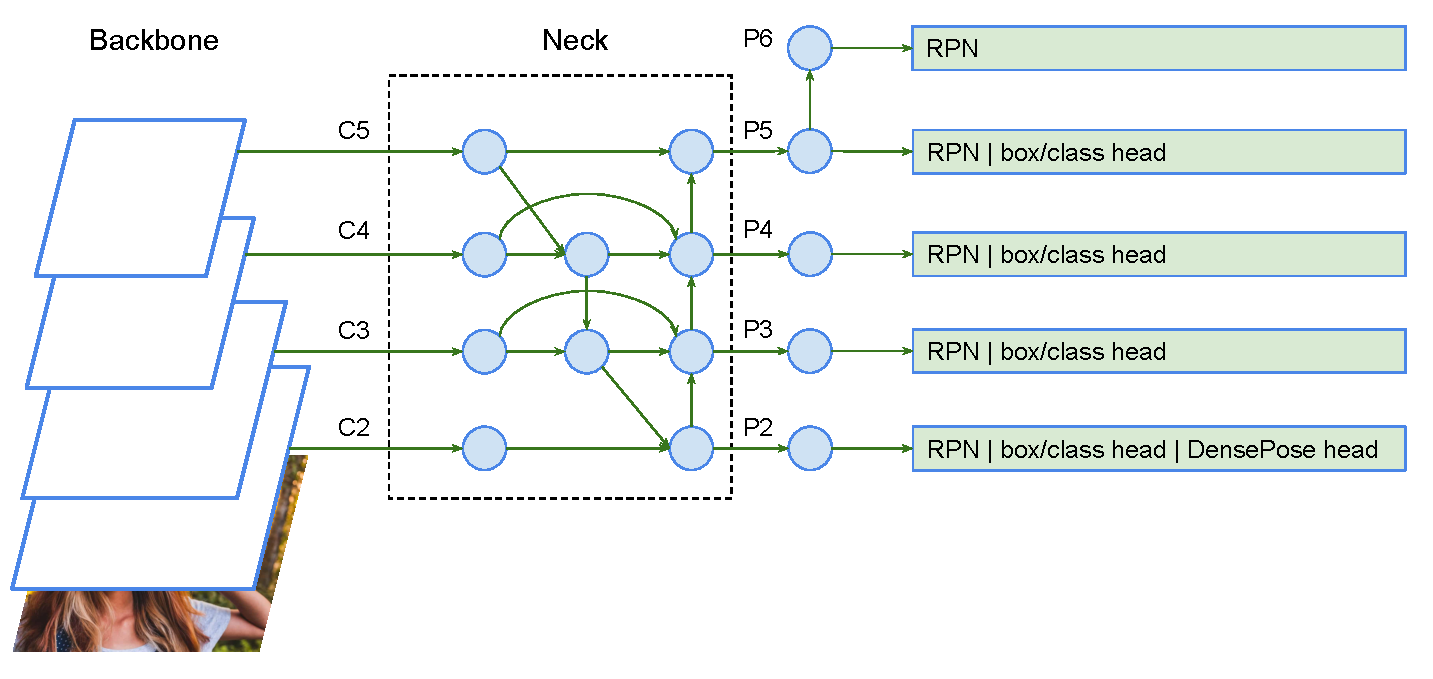
\includegraphics[width=0.4\textwidth]{images/scheme.pdf}
\caption{The high level structure of the Mobile Parsing R-CNN model. $C_i$, $P_i$ represent feature levels with a resolution of $1/2^i$ of the input image. $P_6$ is obtained via stride-2 pooling on $P_5$.}
\label{fig:scheme}
\end{figure}

\section{Dataset}
\label{sec:dataset}

\begin{figure}[!t]
\label{fig:dataset_teaser}
\centering
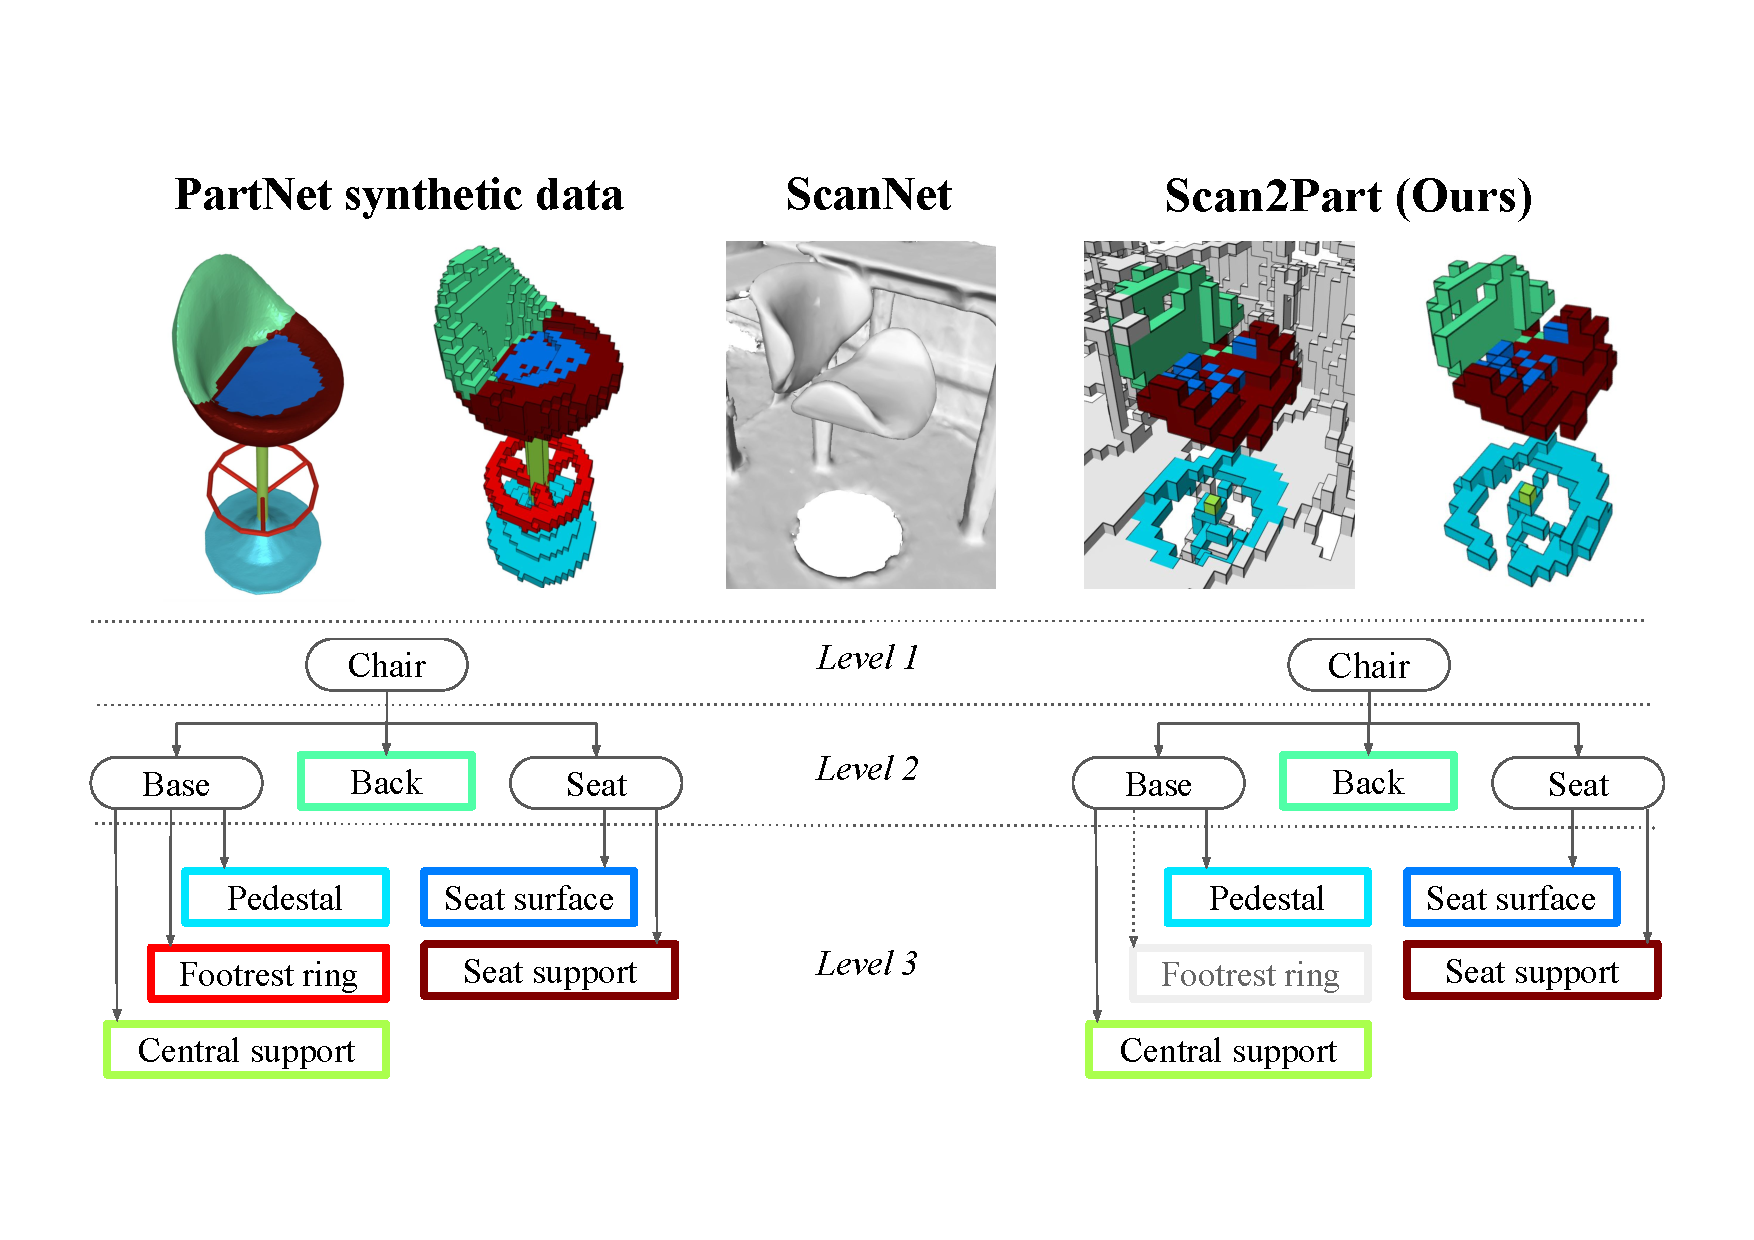
\includegraphics[width=0.99\textwidth]{Figures/scan2part/dataset_teaser.pdf}
\caption{Top:our dataset is obtained by combining PartNet synthetic data with ScanNet sensor data. Bottom: the PartNet object hierarchy is compressed to include only parts sufficiently well represented in ScanNet data.}
\end{figure}

Our first objective is to develop a large-scale 3D scene understanding dataset with part-level annotations. 
We use the 3D geometry in 1,506 3D scenes in ScanNet dataset~\cite{dai2017scannet} reconstructed from RGB-D scans in the form of truncated Signed Distance Function (SDF) at voxel resolution = 3\,cm.
For labeling the scan geometry, we use the parts taxonomy in PartNet dataset~\cite{mo2019partnet} represented as a tree structure where nodes encode parts at various detail levels and edges encode the ``part of'' relationship.
We associate to each 3D scene a per-voxel mask storing leaf part IDs from the taxonomy (i.e., the most fine-grained categories).
To label the 3D scene at a given level~$d$ of semantic detail ($d = 1$ meaning whole objects and $d = 8$ meaning finest parts), we start with the leaf labels in each voxel and traverse the taxonomy tree until hitting depth~$d$.



We further describe the main steps taken to create our Scan2Part benchmark below, leaving the detailed discussion of the technicalities for the supplementary. 
% \DZ{This figure is commented out}
Annotation schema for our dataset is shown in Figure~\ref{fig:dataset_schema}.

\paragraph{Transferring labels to volumetric 3D grids.} 
% \LA{add something about semantic correspondences, ie WHICH object must be where}
To obtain ground-truth semantic parts annotations for real-world 3D scenes, we establish  correspondences between each volume in the 3D scene in ScanNet and a set of part-annotated mesh vertices in a registered 3D CAD model from PartNet.
To this end, we first find accurate 9 degrees of freedom (9\,DoF) transformations between PartNet 3D models and their original versions from ShapeNet, and next use the manually annotated 9\,DoF transformations and their respective object categories provided by Scan2CAD to obtain the final scan-to-part alignments.
We further perform a simple majority voting, selecting only the most frequent (among the vertices) part label as the ground truth voxel label, see Figure~\ref{fig:scan2part_labels_transfer}.
% \LA{how many classes typically fall into this selection and get suppressed in this procedure?}

\begin{figure}[!h]
\label{fig:scan2part_labels_transfer}
\centering
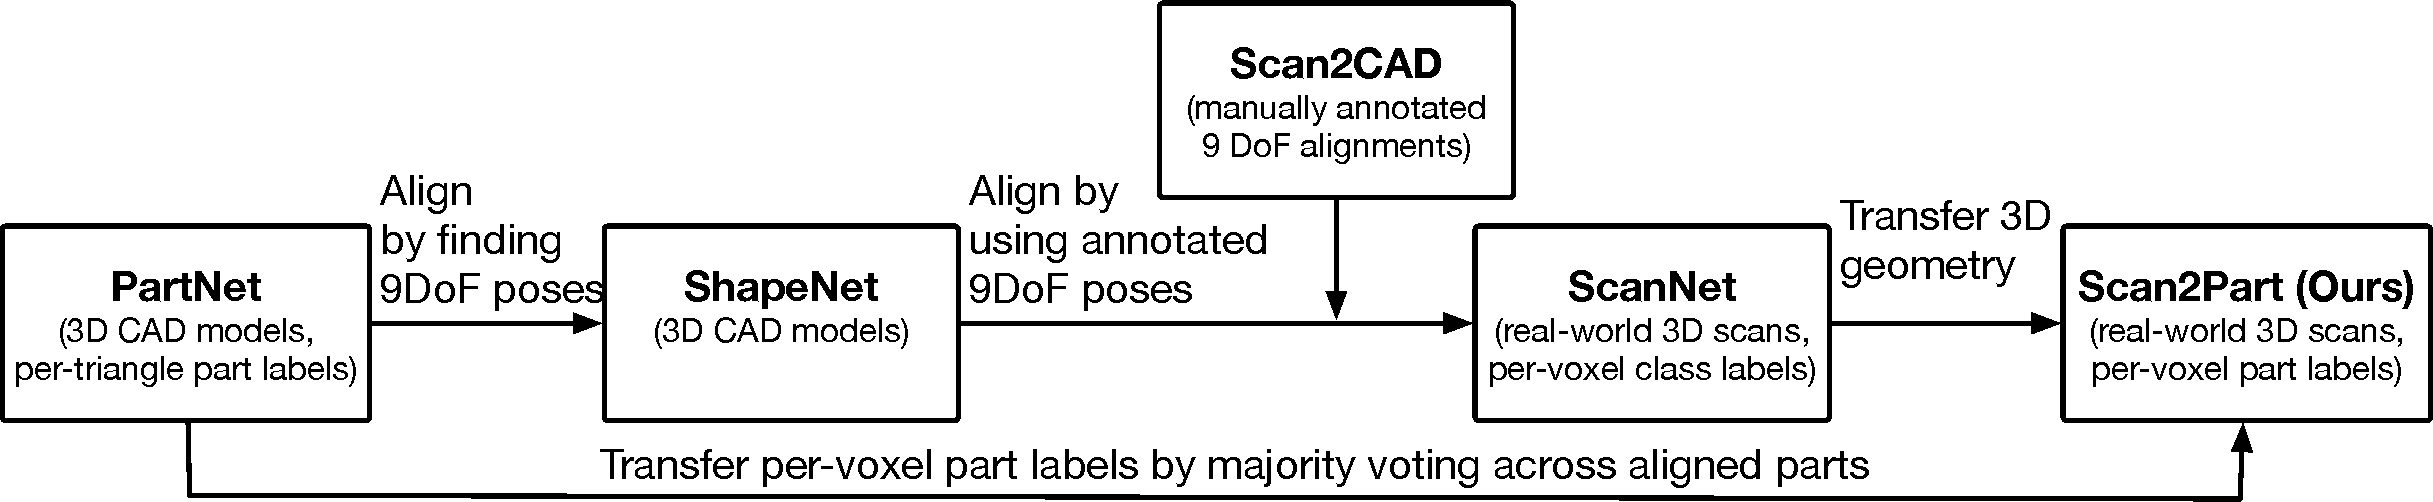
\includegraphics[width=0.99\textwidth]{Figures/scan2part/scan2part_labels_transfer.pdf}
\caption{Our automatic pipeline for part-based 3D scan annotation (see surrounding text).}
\end{figure}


% For this procedure to operate, one needs to register a set of 3D shapes to scans.
% Our resulting Scan2Part dataset consists of

This procedure results in 242,081 correspondences represented as 9\,DoF transformations between 1,506 reconstructions of real-wold ScanNet scenes and 53,618 unique parts of 2,477 ShapeNet objects.
Parts of each object have a tree structure, similar to~\cite{mo2019partnet}.
Note that the majority-based voting implementation of annotation transfer results in some semantic parts labels not being represented in the 3D scan, ultimately affecting parts taxonomy, which we discuss below. 

% we could sample or somehow ensure that at least some representatives of all classes exist in the dataset
% however, we have chosen the simplest implementation in the form of the simple majority voting 
% this results in some classes being omitted due to the finite scan resolution
% in the end, this affects part hierarchy

\begin{figure}[!t]
\label{fig:dataset_schema}
\centering
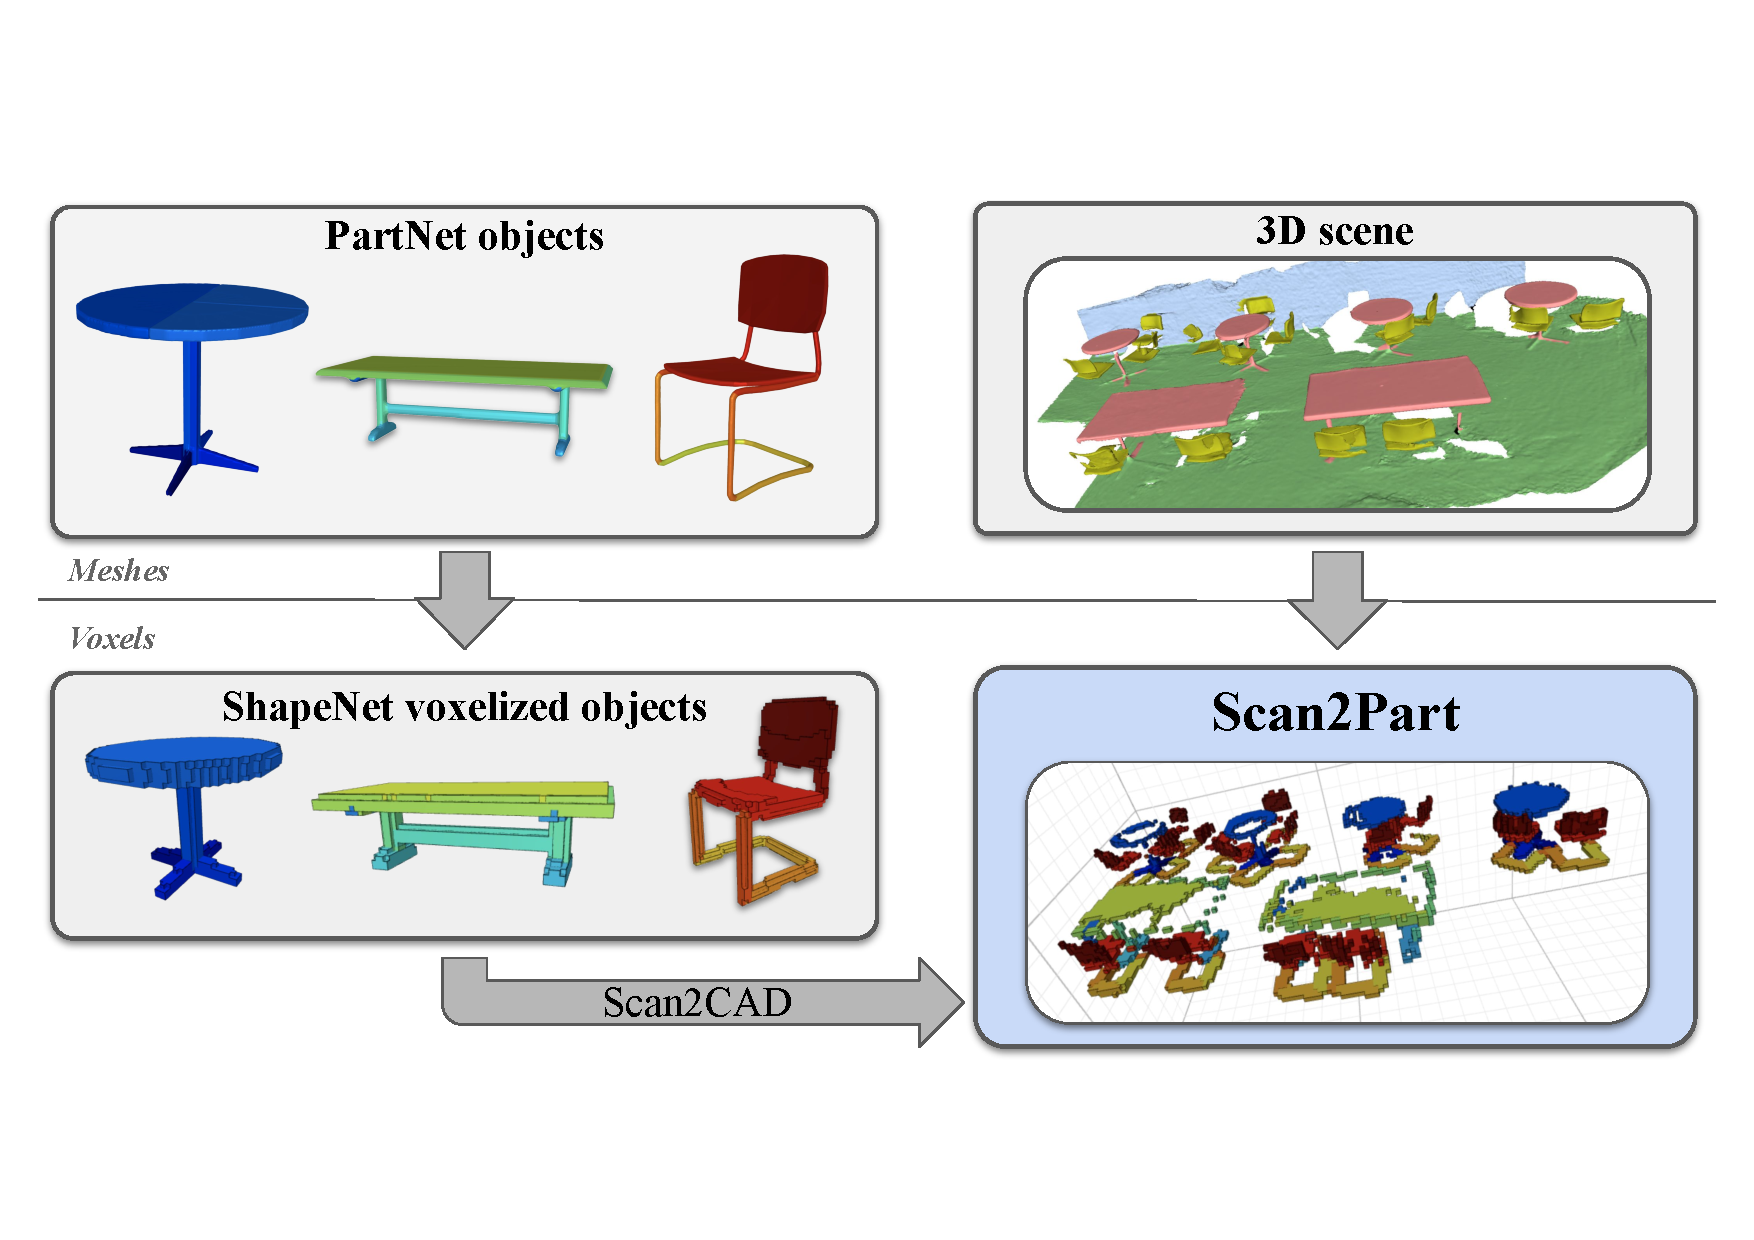
\includegraphics[width=0.9\textwidth]{Figures/scan2part/dataset_schema.pdf}
\caption{A pipeline for obtaining Scan2Part dataset. We project the PartNet \cite{mo2019partnet} labels to the ShapeNet \cite{chang2015shapenet} coordinate system (left), then use Scan2CAD \cite{avetisyan2019scan2cad} dataset to map labels to real scenes from Scannet \cite{dai2017scannet} (right).}
\end{figure}



% \begin{figure}[!t]
% \label{fig:part_level_variation}
% \centering
% 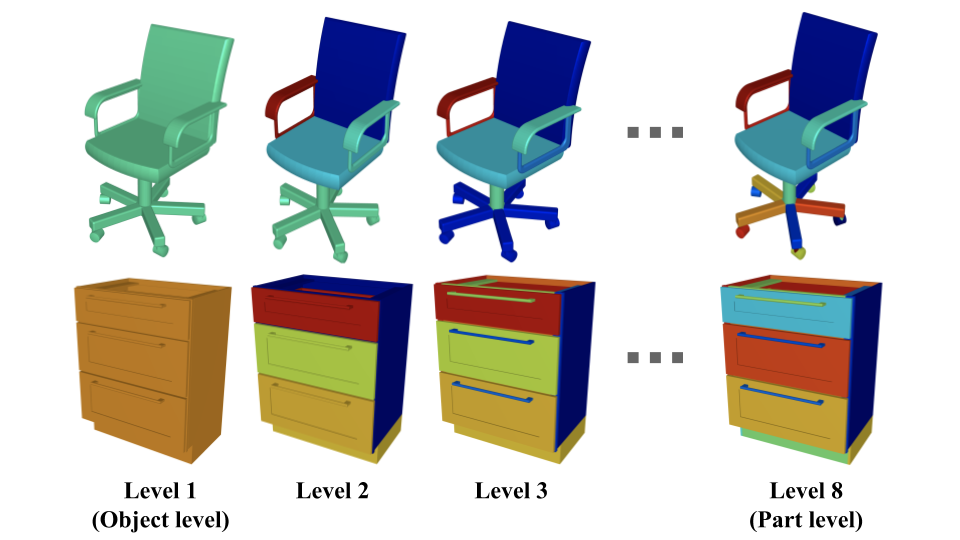
\includegraphics[width=\textwidth]{Figures/scan2part/part_level_variation.png}
% \caption{The object level of detail depending on the part taxonomy tree level based on PartNet taxonomy~\cite{mo2019partnet}. The level of detail  increases from left to right, starting with the object level.}
% \end{figure}

\paragraph{Parts taxonomy processing. } 
% % 1. description of the taxonomy
% % issue: classes that are not represented in 3D scans
% % 2. compressing taxonomy by merging classes
% % 3. compressing taxonomy by pruning the taxonomy tree
% % say something about taxonomy 
The taxonomy of 3D shape parts is represented as a single tree structure based on~\cite{mo2019partnet}. However, as the voxel resolution of the real-world 3D scan is relatively coarse, particular part categories (e.g., small shape details such as keyboard buttons or door handles) cannot be represented by sufficient number of 3D data points, thus implying a reduction in the original taxonomy. 
We proceed with this reduction by first choosing an appropriate occurrence threshold (we pick 1800 voxels, but demonstrate the effect of different threshold values in the supplementary) and remove classes that have smaller number of representatives in the dataset.
% % there are at least 1800 voxels labeled with this part\DZ{why 1800?}  in the entire dataset.
We finalize the taxonomy by pruning trivial paths in the tree (i.e., if a vertex has only one child, then we delete this vertex by connecting the child and the parent of this vertex), but keeping the leaf labels intact. We display the number of vertices at different granularities in the original and resulting part taxonomy levels in Table~\ref{tab:label_presence}.  
Some parts (leafs in the part taxonomy) are not represented in ScanNet data, so we remove these from the tree. 
% At the first tree level, each tree node  represents an entire object (bed, chair, table, etc.), at the second tree level --- the object base components (bed base, soft part, etc.), and so on.  An example of coloring an object by parts for different taxonomy levels is shown in the figure~\ref{fig:part_level_variation}
% %Each tree level is a level of object details: the deeper the tree level, the more detailed the parts division becomes.

% % we project partnet into scannet not vice-versa 
% % one could have done the other way around, e.g. say use subdivision (octrees) and place "ideal" CAD models into the scannet scenes, preserving ALL partnet classes 
% % but we're specifically interested in preserving as much as possible of the scannet noisy geometry 
% % additionally overlap between partnet and scannet categories is lower than 100%

% To build the part taxonomy, we choose the rules for combining the part trees of all the objects represented in Scan2Part. The total number of all instance parts is 242,081, while there are 53,618  unique parts (figure~\ref{fig:three_tables}, left).
% This is an extremely large number of labels for part segmentation, so we have to apply a more intelligent combination of part trees of different objects.
% If we assume that there are identical parts inside the same object, e.g., four table legs are four instances of the ``leg'' part (figure \ref{fig:three_tables}, center), then the total number of unique parts is reduced to 14,782. It is worth noting that in this case, the legs of different tables will be represented as different parts.

% However, if we assume that there are identical parts inside the same object class, i.e. all the legs of all tables are instances of ``leg'' part (figure \ref{fig:three_tables}, right), then the number of unique parts is reduced to 307.  

% % \DZ{It is unclear from the above what the rules actually are. It says if we assume this, then .., and if we assume that, then ...  Please state what exactly the rules are, and then explain why, e.g., to reduce the number of classes (and why this is a good thing)}

% Some parts (leafs in the part taxonomy) are not represented in ScanNet data, so we remove these from the tree. 
% A particular part is considered sufficiently represented if amount of voxels in the entire dataset labeled with this part is above certain threshold. 
% Through analysis of labels distribution we chose our threshold to be equal to 1800 voxels, but demonstrate the effect of different threshold values in the supplementary.
% % there are at least 1800 voxels labeled with this part\DZ{why 1800?}  in the entire dataset.
% After cleaning the tree, we get rid of trivial paths in the tree (if a vertex has only one child, then delete this vertex by connecting the child and the parent of this vertex) \DZ{what happens to labels?}  The number of vertices at different part taxonomy levels is shown in the table \ref{tab:label_presence}. 
% (\textcolor{red}{why do we use the first 3 levels?})

% \begin{figure}[!t]
% \label{fig:three_tables}
% \centering
% 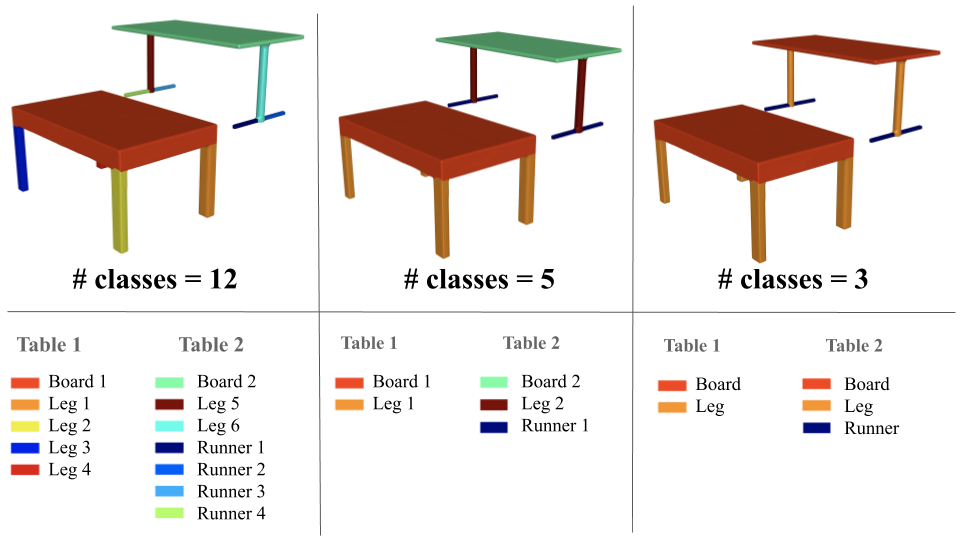
\includegraphics[width=0.9\textwidth]{Figures/scan2part/three_tables}
% \caption{Different rules for combining the part trees of all the objects. \textcolor{red}{TODO}: more specific. (left) if colors of all the legs are different, (center) if color of legs depends on the the table, (right) if color of all legs are the same.}
% \end{figure}


% \begin{figure}[!t]
% \label{fig:three_tables}
% \centering
% 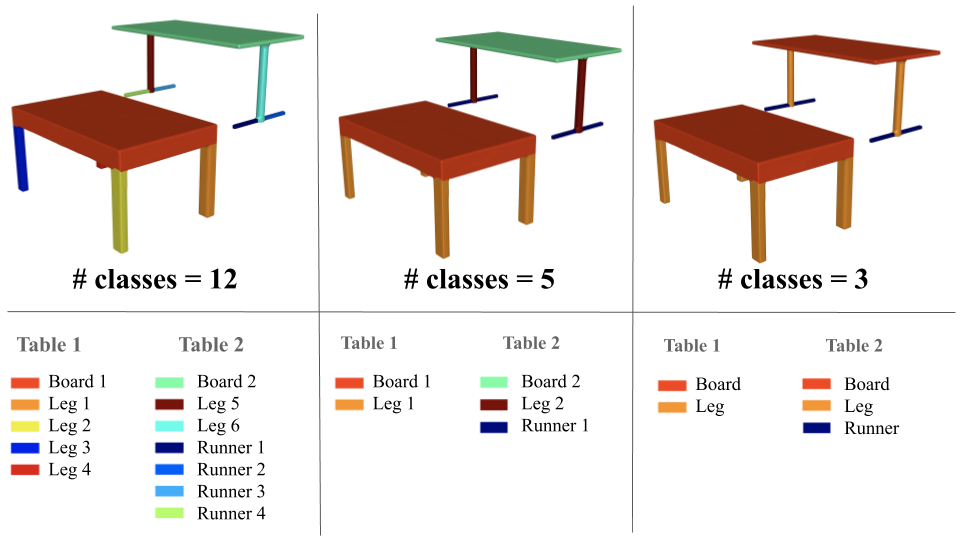
\includegraphics[width=0.9\textwidth]{Figures/scan2part/three_tables}
% \caption{Different rules for combining the part trees of all the objects. \textcolor{red}{TODO}: more specific. (left) if colors of all the legs are different, (center) if color of legs depends on the the table, (right) if color of all legs are the same.}
% \end{figure}





\begin{table}[ht!]
\centering
\caption{Number of parts on each tree level.
% \textcolor{blue}{@alex\_notch please double-check. numbers should be consistent over all the text}
}
\label{tab:label_presence}
\resizebox{0.8\textwidth}{!}{%
\begin{tabular}{l cccccccc}
\toprule
\multirow{2}{*}{\textbf{Level}} & \textbf{1} & \textbf{2} & \textbf{3} & \textbf{4} & \textbf{5} & \textbf{6} & \textbf{7} & \textbf{8} \\
& \textbf{(object)} & & & & & & & \textbf{(part)} \\
\midrule
Full Taxonomy & 18 & 50 & 133 & 223 & 269 & 302 & 306 & 307 \\
Sufficient Taxonomy & 13 & 36 & 79 & --- & --- & --- & --- & --- \\
\bottomrule
\end{tabular}
}
\end{table}


% In the last 4 years the field of computer vision saw an increase in Real-world 3D Scenes datasets acquired using depth sensors and LIDAR's, also level of detalization of object labels have increased, with complete object-part composition tree being the latest achievement~\cite{mo2019partnet}. The object part annotations were applied to meshes of objects that were created digitally and not measured by sensors. To address the problem of detecting object parts in real-world scans we needed a new dataset, so we decided to compose one ourselves from from four different sources.


% \begin{figure}
% \label{fig:dataset_overlap}
%   \centering
% 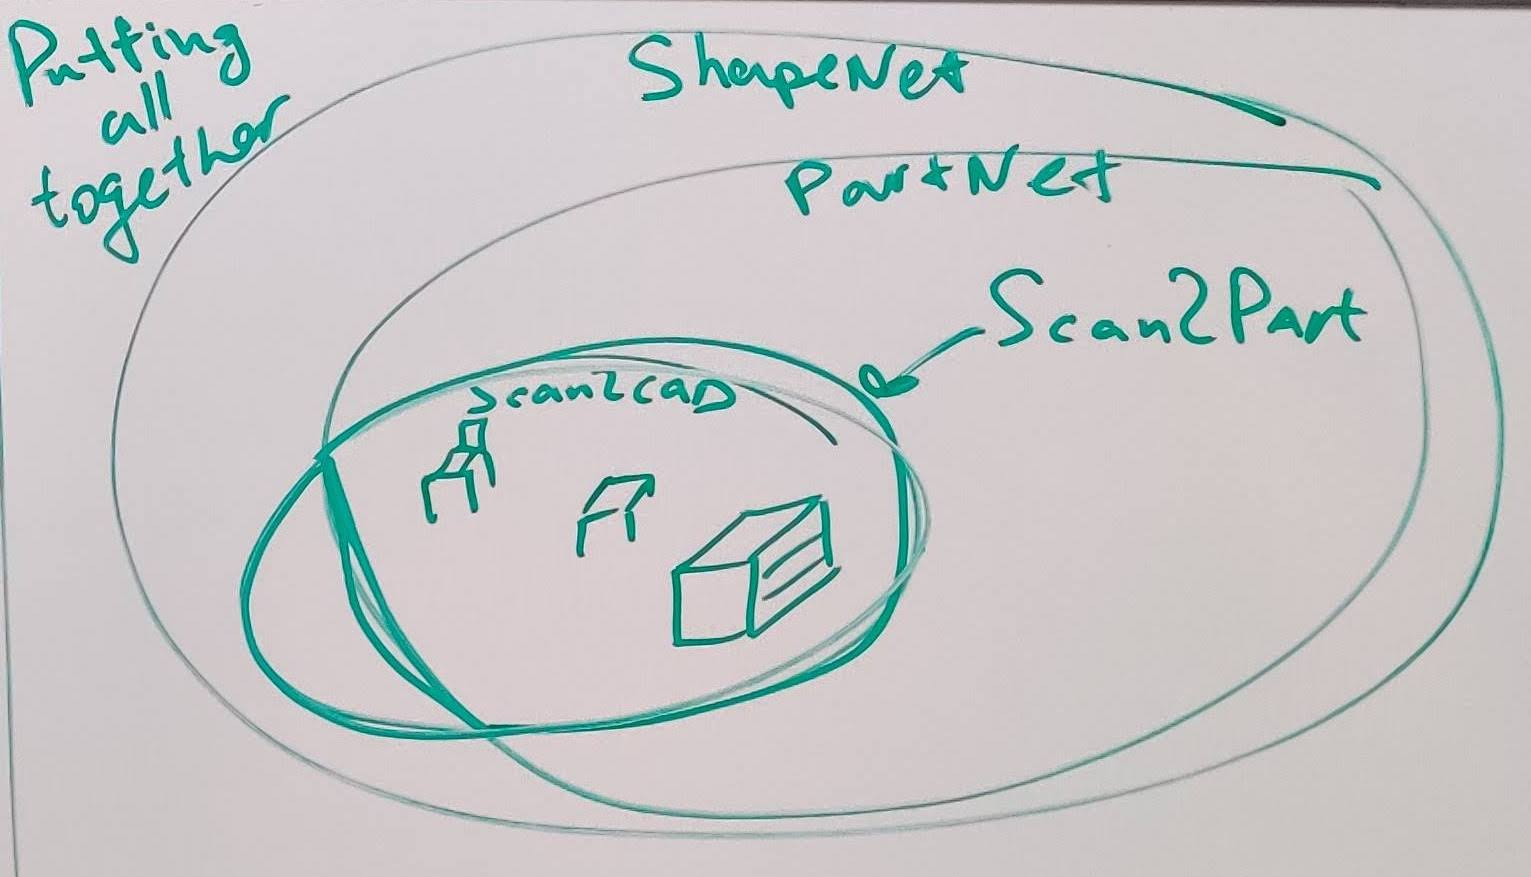
\includegraphics[trim=0 0 0 0, max width=0.5\textwidth]{Figures/scan2part/dataset_overlap.jpg}
% \caption{Venn Diagram of Datasets (PartNet $\subset$ Shapenet, Scan2CAD $\subset$  Shapenet)}
% \end{figure}

% \subsection{Labeling}
% \subsubsection{Shapenet to PartNet}
% \textbf{Projection}
% % \caption{left picture: gray shapenet, right picture: colored partnet}
% \textbf{ICP} 
% % \caption{two histogram of AVG CD between two objects: before and after ICP}
% % \caption{best and worst cases according to previous histogram}
% \subsubsection{Scan2CAD: ScanNet to Shapenet}
% % \caption{example from the Scan2CAD dataset}
% \subsection{Data-driven part taxonomy}

% After joining instance labels to class labels number of elements is reduced first to 53k, then to 20k, and finally to 308 classes.

% After further pruning because 20 of the part classes don't have a single voxel, number of classes can be reduced from 308 to 288 classes.
% % \caption{histogram of voxel appearance on the scenes}
% % \caption{example of prunned classes}
% % \caption{example of good class (not so deep)}
% \subsection{Model-driven part taxonomy}

% \subsection{Scan2Part}
% % \caption{tiser}

% \begin{table}[]
% \centering
% \caption{Dataset funnels}
% \label{tab:dataset_funnels}
% \begin{tabular}{l|l|l|l|l}
%  & Total count & PartNet & Scan2CAD & Scan2Part \\
% \hline
% Scenes from ScanNet & 1.5k & - & 1.5k & 1.5k \\
% Shapes from ShapeNet & 30k & 24k & 3k & 2.7k
% \end{tabular}
% \end{table}

% \begin{figure}
% \label{fig:Partnet_overview}
%   \centering
% % 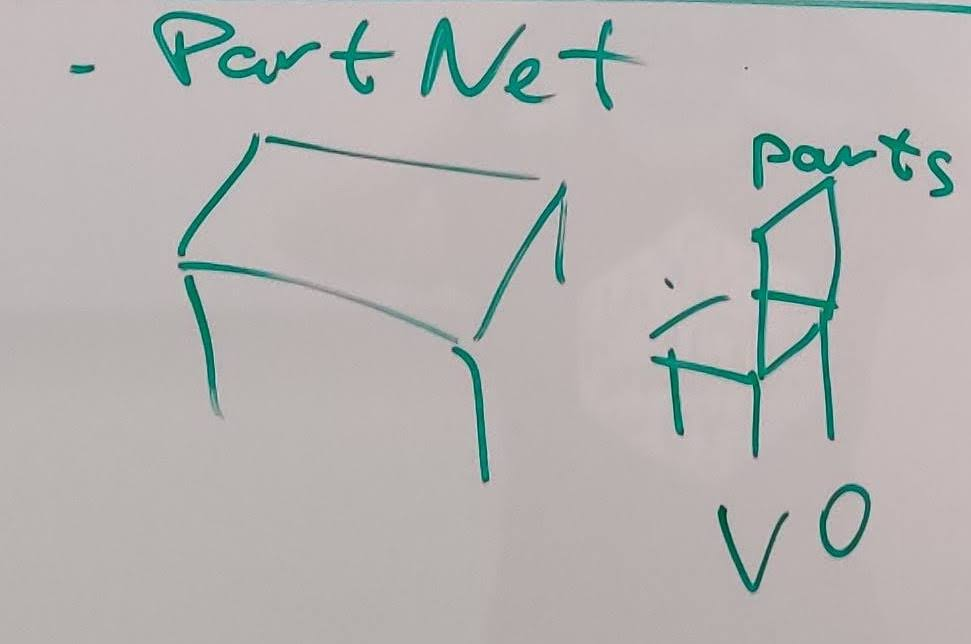
\includegraphics[trim=0 0 0 0, max width=0.5\textwidth, right]{Figures/scan2part/Partnet_overview.jpg}
% 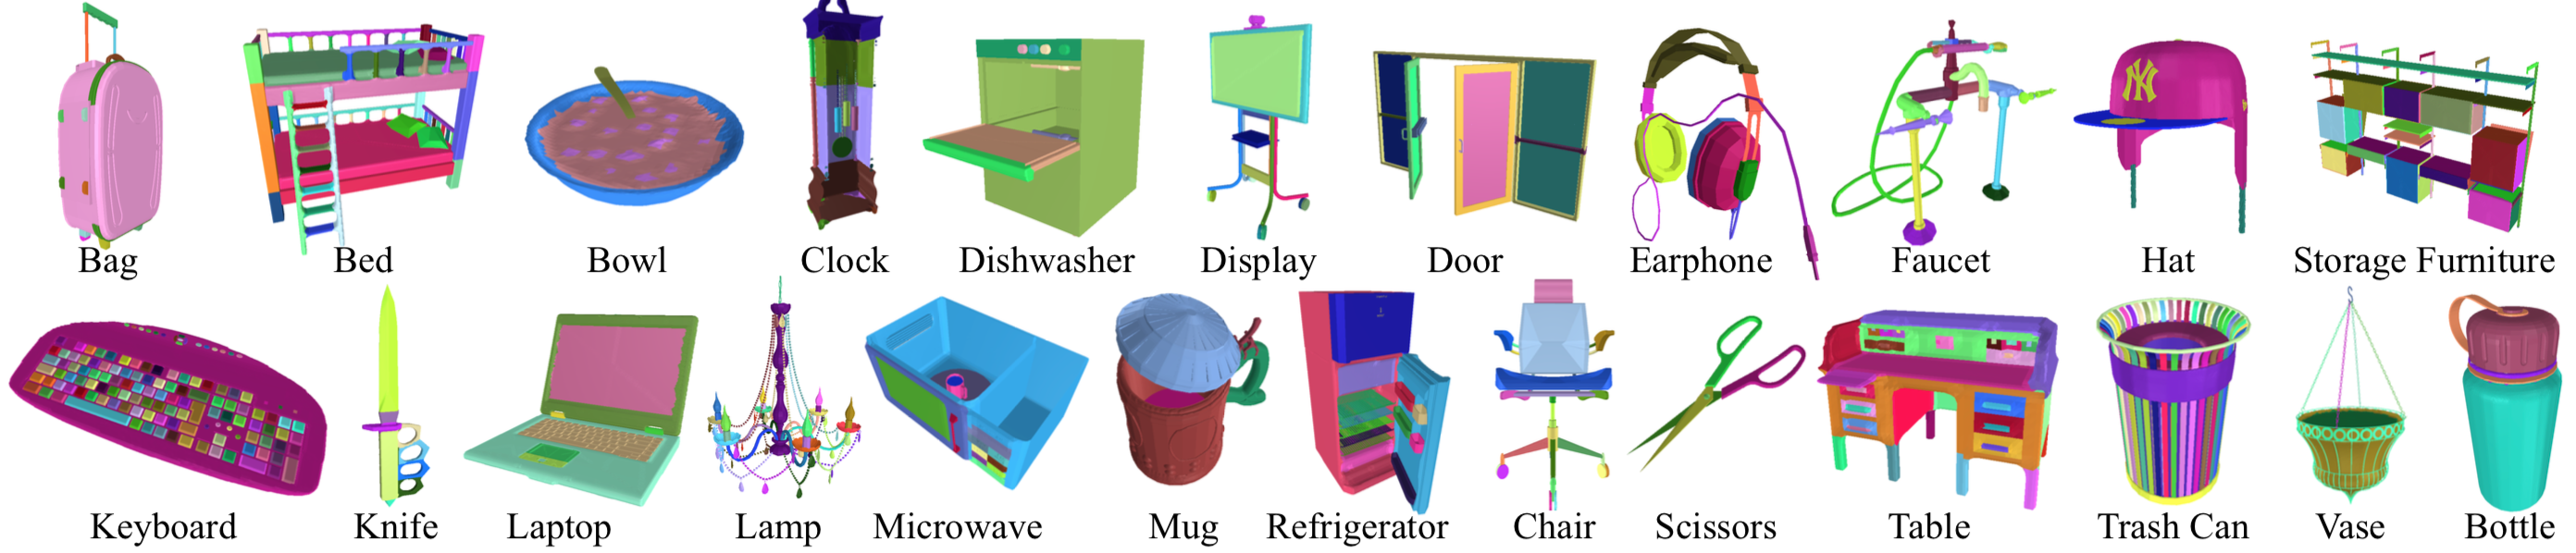
\includegraphics[trim=0 0 0 0, max width=\textwidth, right]{Scan2Part/images/partnet_data_visu.png}
% \caption{Partnet overview}
% \end{figure}

% В изображении~\ref{fig:partnet_to_scannet_labeling}а можно увидеть различие в детальности полигональной сетки в объектах датасетов ShapeNet и PartNet, высокая полигональность - последствие метода разметки деталей объекта в web-интерфейсе.
% На графике~\ref{fig:partnet_to_scannet_labeling}б изображено расспределение метрики Чамфера на соответствующих объектах в датасетах ShapeNet и PartNet, как можно заметить многие формы объектов в своих исходных положениях отличаются значительно. Поэтому для установления общей системы координат требуется решить задачу регистрации, которую мы решаем с помощью метода ICP~\cite{besl1992method}. На графике~\ref{fig:partnet_to_scannet_labeling}в можно увидеть как изменилось расспределние метрики Чамфера, ее высокое значение в некоторых случаях объясняется как нахождение методом ICP локального минимум соответствующему одному из симметричных положений объекта в разных датасетах, и не должно значительно повлиять на перенос разметки в датасет ShapeNet.  

% \clearpage

% % \begin{wrapfigure}{l}{0.25\textwidth}


% \begin{figure}[!htb]
% \label{fig:taxonomy_overview}
% \centering
% 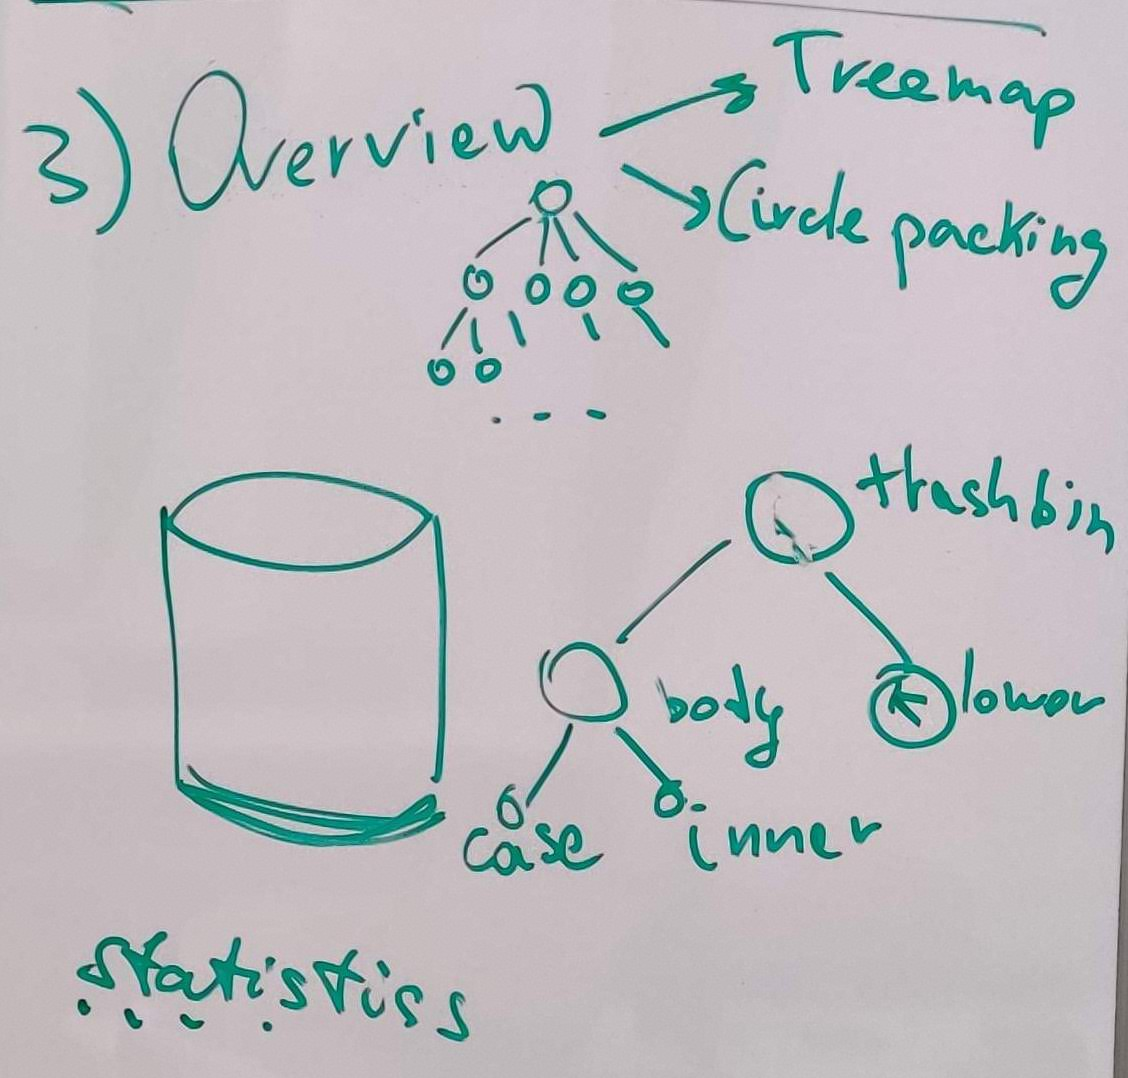
\includegraphics[trim=0 0 0 0, max width=0.5\textwidth]{Figures/scan2part/taxonomy_overview.jpg}
% \caption{taxonomy overview}
% \end{figure}


% \begin{figure}[!htb]
% \label{fig:scan2part_overview}
%   \centering
% 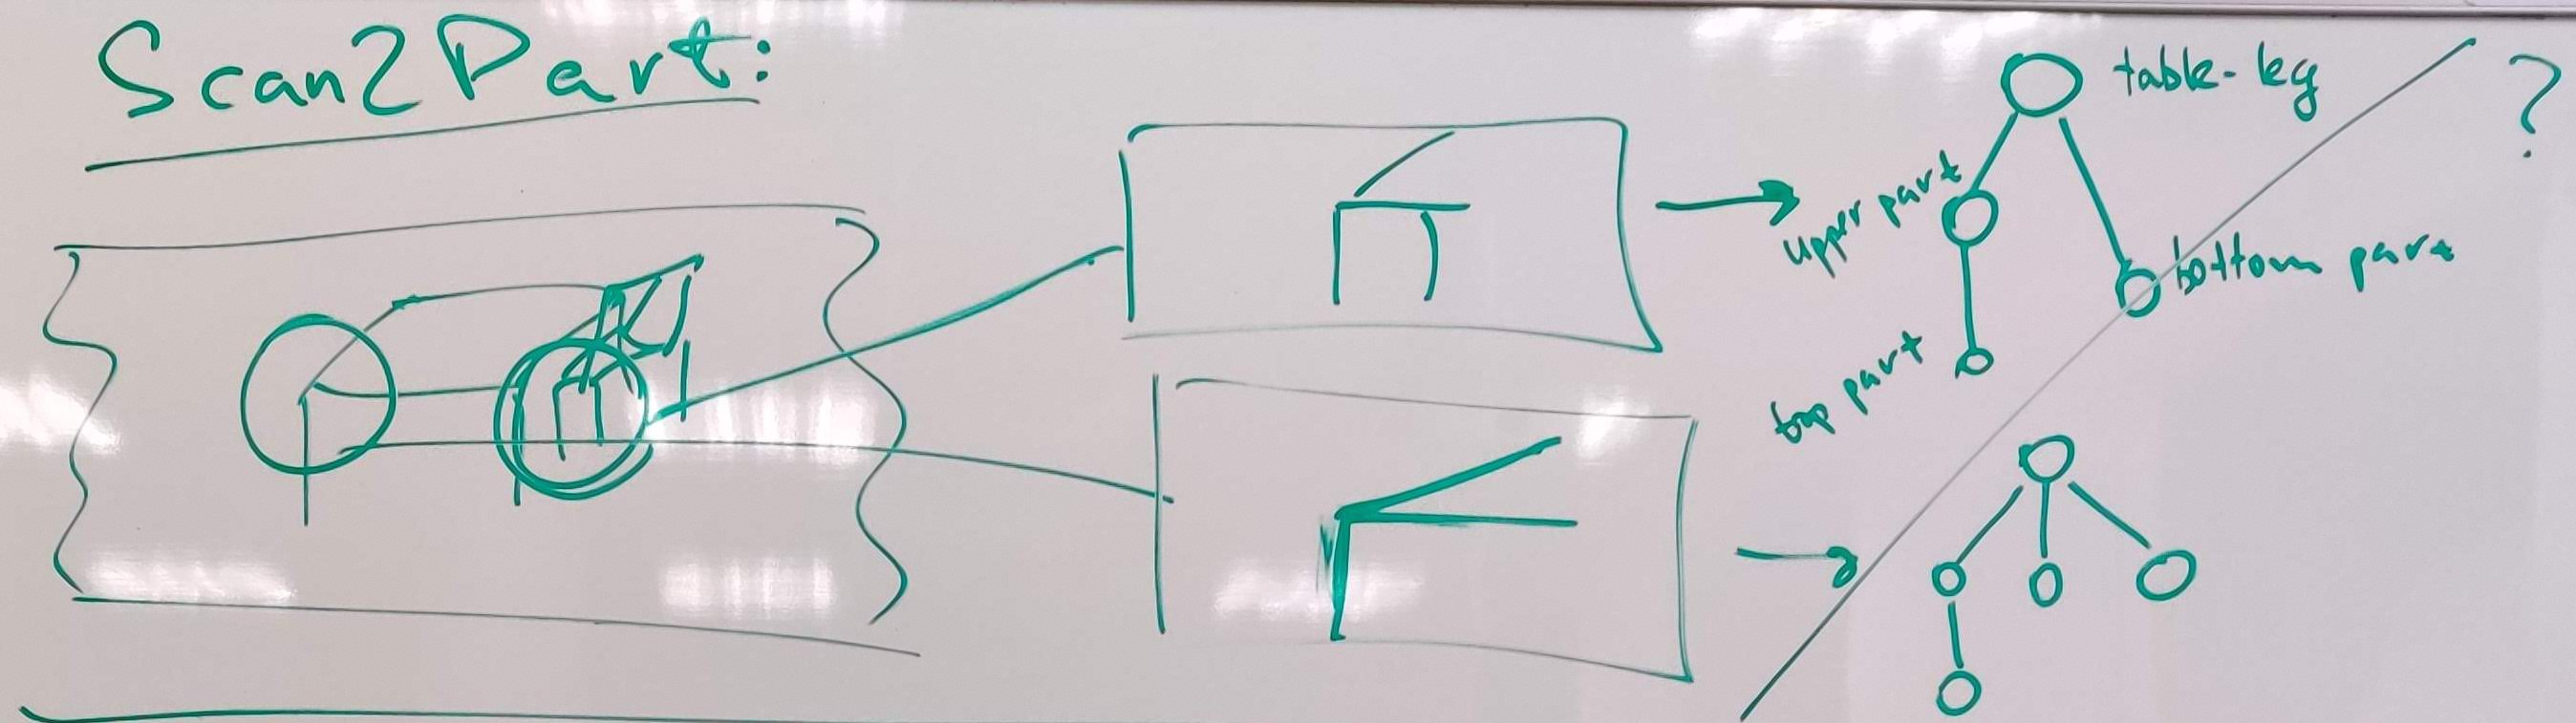
\includegraphics[trim=0 0 0 0, max width=0.5\textwidth]{Figures/scan2part/scan2part_overview.jpg}
% \caption{scan2part overview}
% \end{figure}
% \begin{figure}
% \label{fig:taxonomy_compression}
%   \centering
% 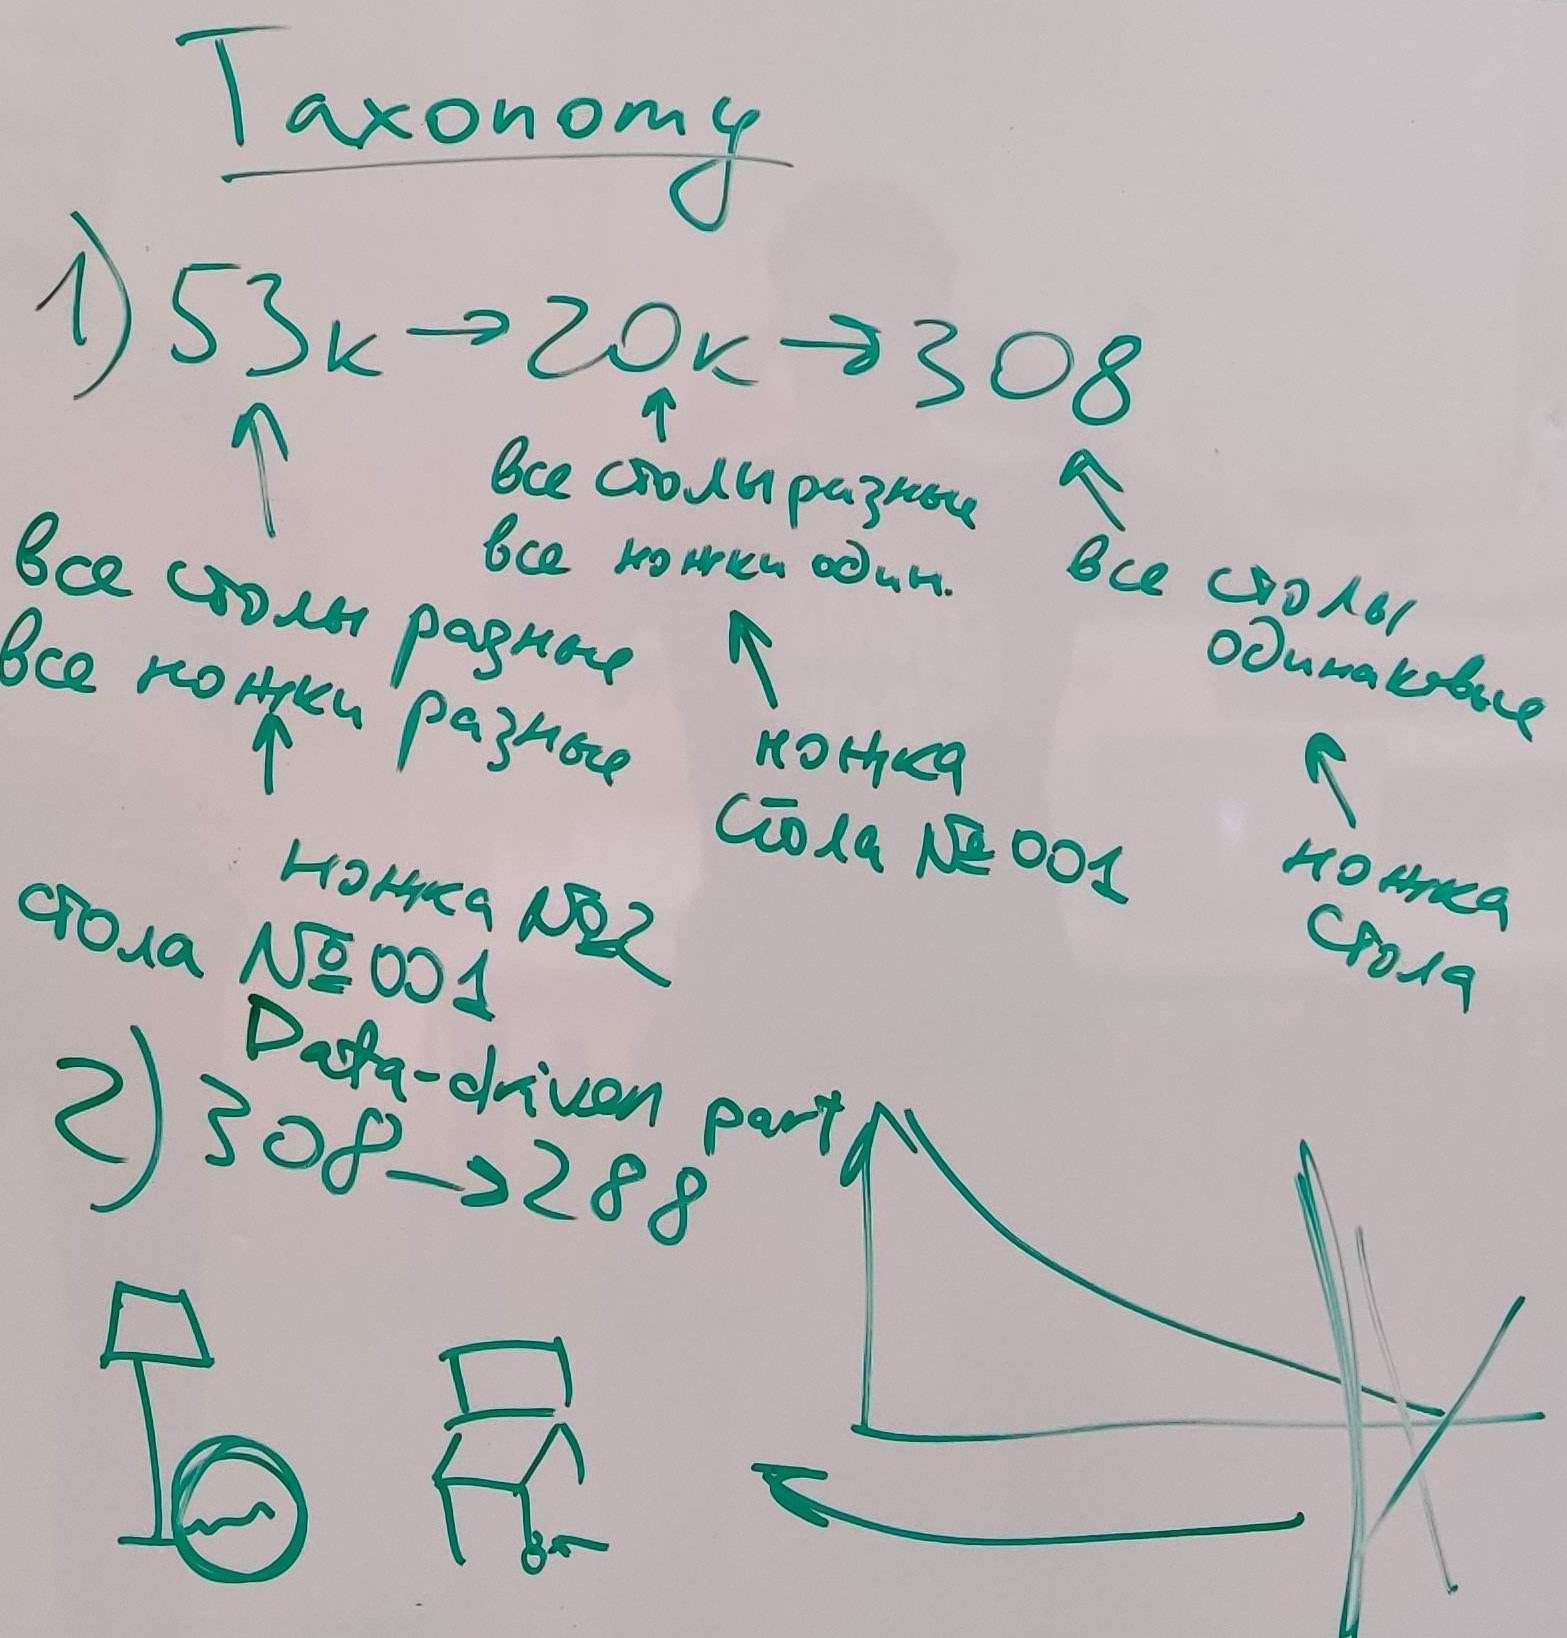
\includegraphics[trim=0 0 0 0, max width=0.5\textwidth]{Figures/scan2part/taxonomy_compression.jpg}
% \caption{taxonomy compression}
% \end{figure}

% \begin{figure}[!htb]
% \label{fig:dataset_mapping}
%   \centering
% 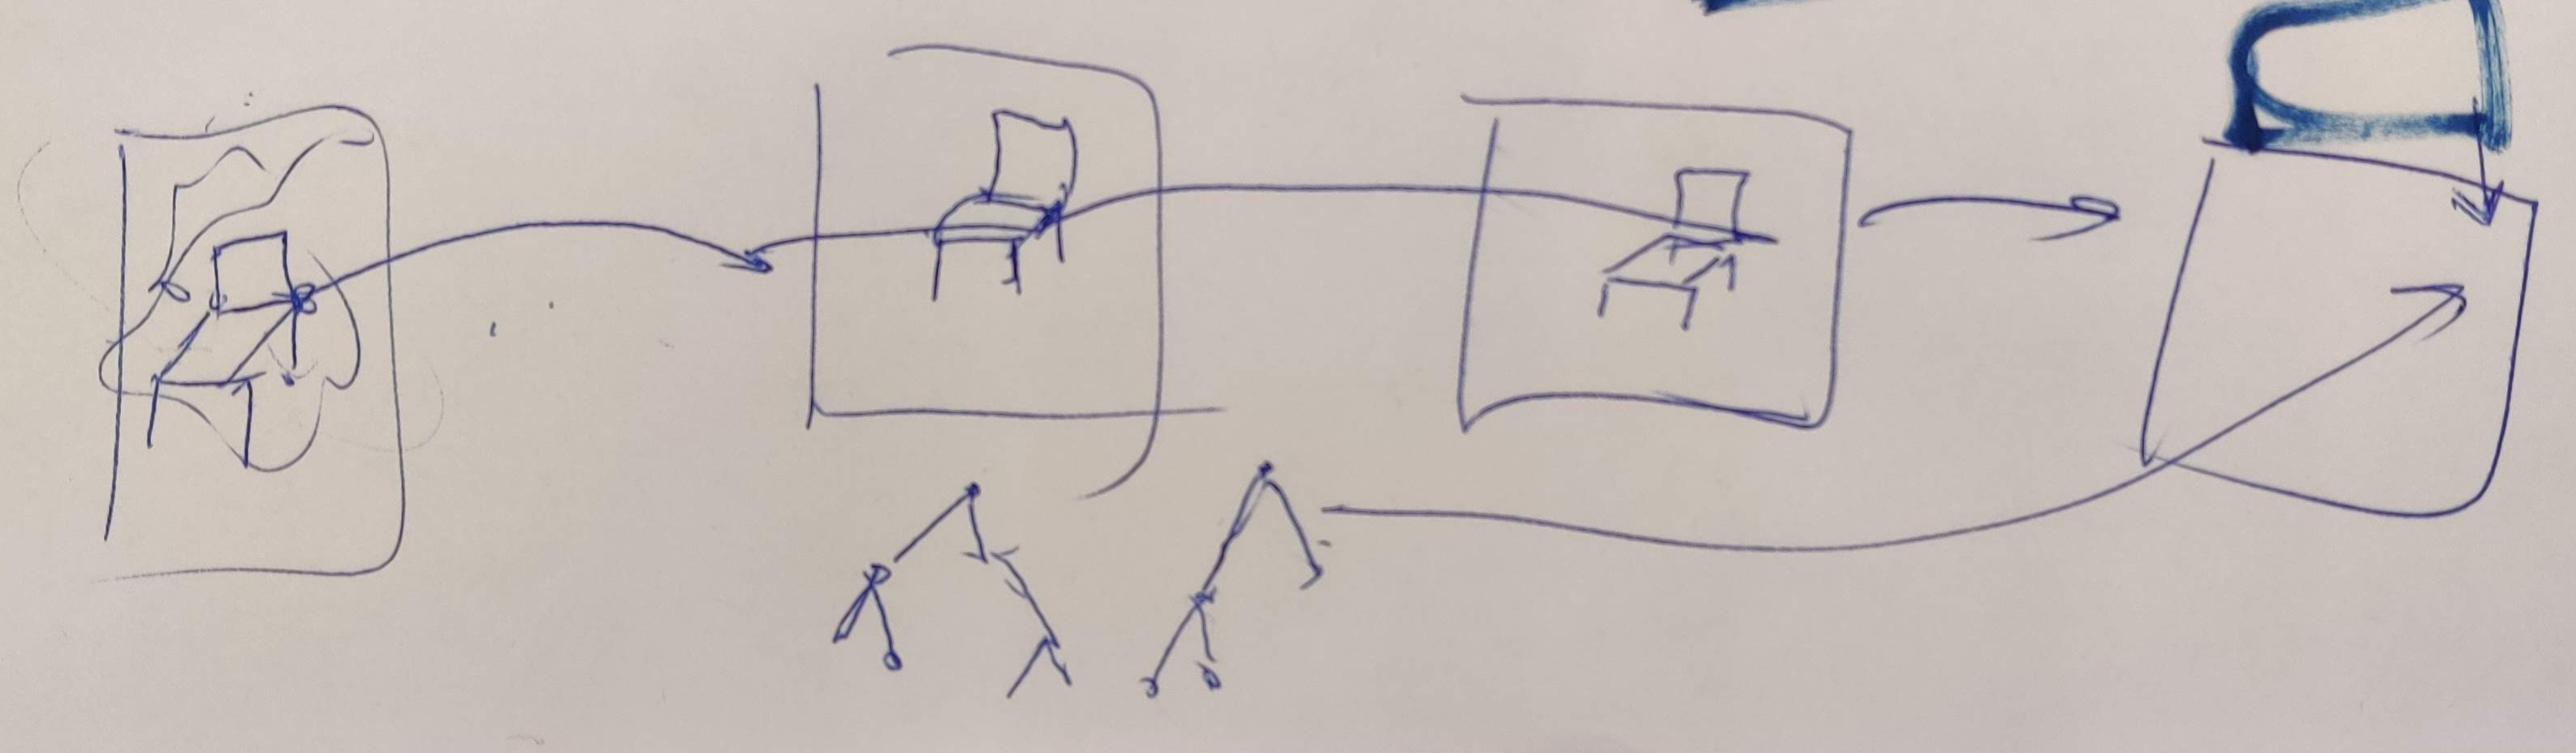
\includegraphics[trim=0 0 0 0, max width=\textwidth]{Figures/scan2part/dataset_mapping.png}
% \caption{Mapping of voxels in ScanNet scene to CAD model and to part hierarchy of the object}
% \end{figure}


% % \subsection{Scan2Part dataset preparation}
% The ScanNet \cite{dai2017scannet} is a dataset of RGB-D scans of real-world indoor scenes with multiple kinds of data representation and semantic object-level labels for those scans.
% The Scan2CAD \cite{avetisyan2019scan2cad} is a dataset that alignes CAD objects from ShapeNet \cite{chang2015shapenet} database to scenes from Scannet, therefore serving as a connective tissue to labels.
% The PartNet \cite{mo2019partnet} is a hierarchical instance level parts dataset of labeles for subset of ShapeNet database. The PartNet dataset the only dataset that has deep hierarchical structure compared to other part annotation datasets like in \cite{Yi16}.

% Using marching cubes algorithm we obtained a voxelised version of scenes from ScanNet dataset with object type labels and mapping of coordinate systems from ScanNet to ShapeNet, because of that we can calculate position of CAD object parts in the scene coordinate system and calculate relative volume in specific voxels thus projecting part labels on scene. 
% Under closer examination we discovered that most of the parts don't have a unique shape making task of instance segmentation for parts very hard to solve and not necessary for practical scene segmentation task.





% 
% 4) При решении собственно задачи понимания сцены на уровней частей естественно возникает некоторая иерархическая структура разметки. 
% — Выбор таксономии играет решащую роль при сегментации, так как слишком грубые таксономии будут неотличимы от просто сегментации и потому бесполезны, а слишком детальные не реализуются из-за ограничений разрешения и шума. 

% \begin{figure}[!t]
% \label{fig:dataset_teaser}
% \centering
% 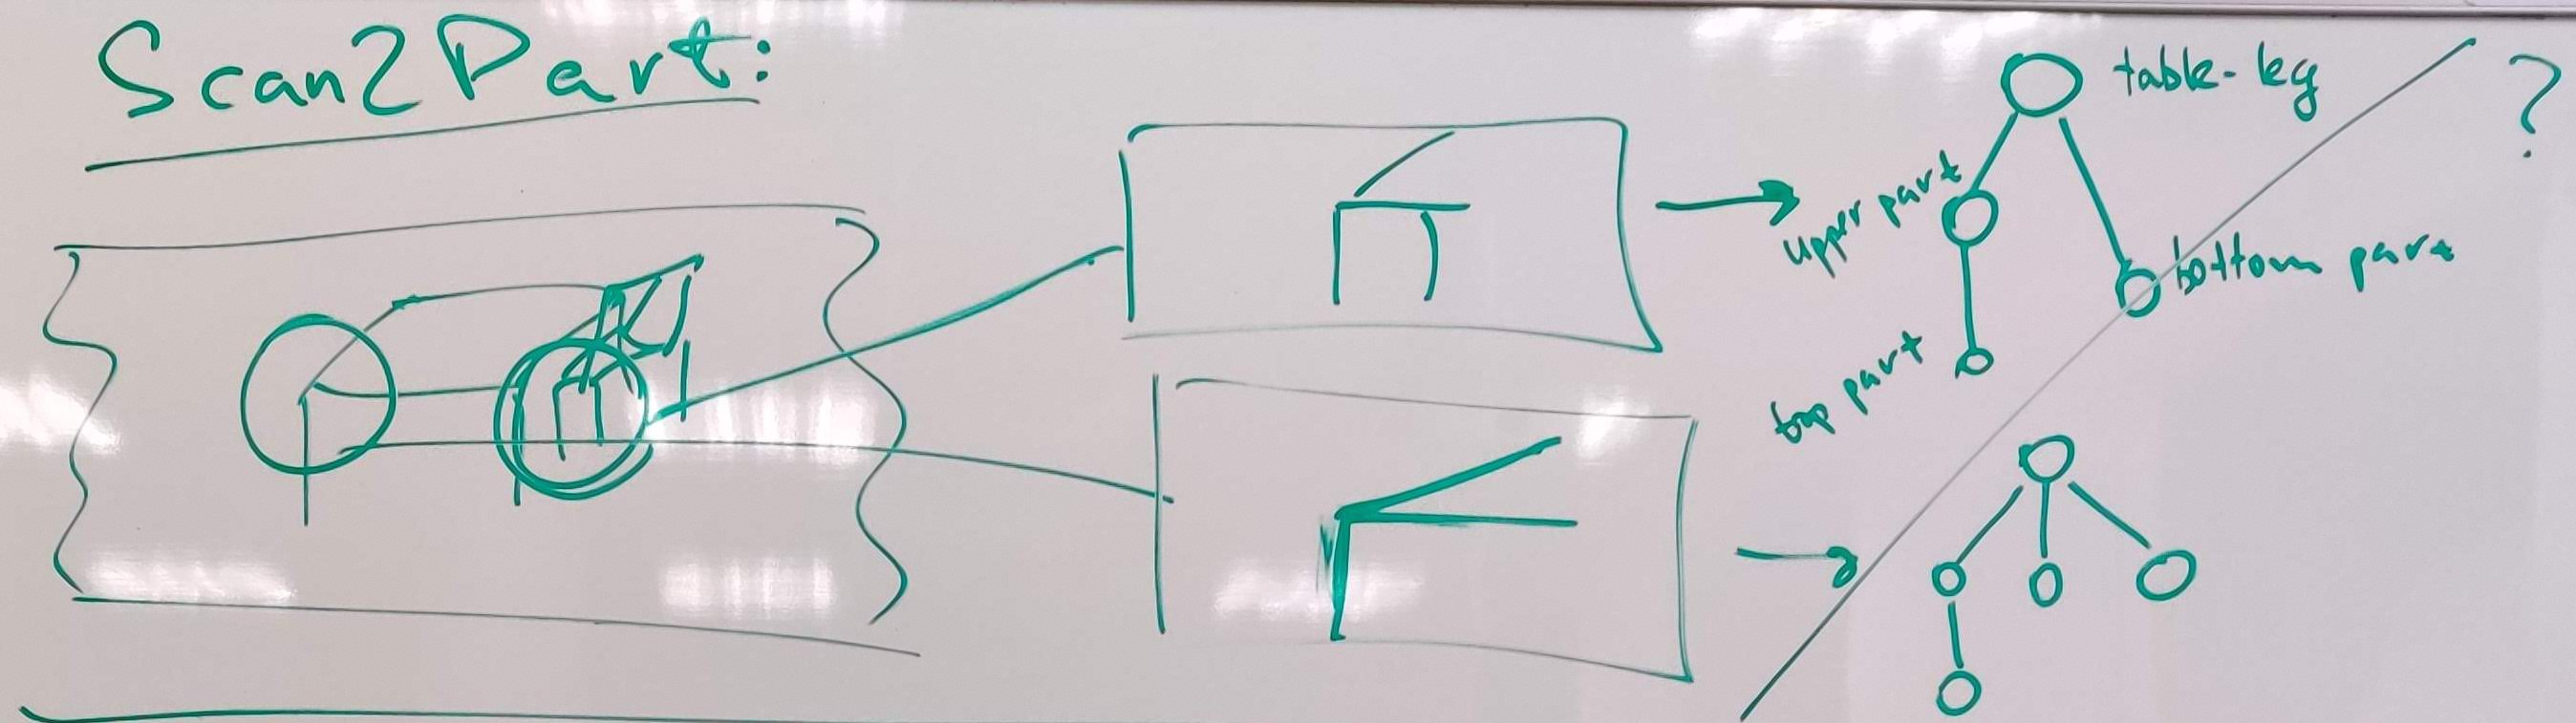
\includegraphics[width=0.9\textwidth]{Figures/scan2part/scan2part_overview.jpg}
% \caption{Dataset teaser}
% \end{figure}

%


% \textcolor{red}{TODO}: Table with abovementioned numbers.



\section{Methodology}
\label{sec:methods}

\paragraph{Classes of 3D understanding tasks. }
\label{methods:tasks}
We consider three distinct classes of challenging part-level 3D scene understanding tasks: semantic labeling, hierarchical semantic segmentation, and instance segmentation. 
The input to all our models is the voxelized scene SDF, representing 3D geometry without associated RGB values.

In~\emph{semantic labeling,} the goal is to associate a set of $n$ semantic part labels~$y_j = (y_j^{d_1}, \ldots, y_j^{d_n})$ with each voxel~$v_j$, 
at detail levels~$d_1, \ldots, d_n$.
To predict parts in such multi-label formulation, we produce a set of softmax scores $p_j = (p_j^{d_1}, \ldots, p_j^{d_n})$.
We train the network in multiple setups, differing by the structure of supervision available to the network, each time evaluating labeling performance at each detail level $d_i$. Specifically, we define 
our loss function $L$ to be a weighted sum of cross entropy losses for each level of detail
\begin{equation}
\label{eq:semseg_loss}
L(p, y) = \sum_{k = 1}^K \alpha_k L_{\text{CE}}(p^k, y^k)
\end{equation}
and specify a set of weighting schemes for $\alpha_1, \ldots, \alpha_K$. 
This loss structure allows expressing both ``flat'' segmentation formulations (e.g., choosing $\alpha_{k} = \delta_{ki}$ to segment at level $d_i$ only), that we view as baselines, and multi-task formulations that integrate training signal across multiple levels of semantic detail.

For this task we 

To perform \emph{hierarchical semantic segmentation,} one must perform segmentation at multiple levels in the hierarchy, inferring labels in coarse- and fine-grained detail levels simultaneously. 
Similarily to~\cite{mo2019partnet}, we approach this task using \emph{bottom-up,} \emph{top-down} and \emph{ensemble} method.
Bottom-up method performs segmentation at the most fine-grained level and propagates the labels to object level, leveraging the taxonomy structure.
Conversely, the top-down approach infers labels first at coarse level (starting with objects) and subsequently at finer levels (parts), recursively descending along predicted taxonomy branches.
With the ensemble method, predictions of networks independently trained at distinct detail levels are integrated in a joint inference step.
We note that \emph{multi-task training} using~\eqref{eq:semseg_loss} also results in a hierarchical segmentation method, and include it in the comparison.






% we use a set of linear layers and project voxel features to labels, producing

% The model assigns the input  to several classes \DZ{unclear -- one of several classes?  what is depending on what?}  depending on the total number of part classes on the selected level of detail (LoD) of objects part taxonomy.
% The distribution of class labels on all of LoDs is very unbalanced, as shown on the treemap diagram \ref{fig:class_distribution_treemap}.
% On a given level of detail $k$, the frequency of  a voxel class $i=0 \ldots N^k$ is denoted $C_i^k$.  Then the Cross Entropy loss function weights for class $i$ are equal to $w_i^k = \frac{\max_{i=0 \ldots N^k} (C_i)}{C_i}$.
% If the model is trained to predict labels for several levels of detail $\{k,n,p\}$ we use multiple linear layers to project each voxel features to labels. The final loss function $L$ is computed as a weighted sum of Cross Entropy losses for each level of detail: 
% \[L = \sum_{j\in\{k,n,p\}} w_j L_j
% \]

% flat softmax at lod=1,2,3, and multiloss(12, 123), with quality computed separately (+bottom up deduced labels), +topdown with own softmax labels with masking all of the other labels: here inference would be, choose heads which are predicted as positive, and go one level down inferring, ensemble 


% — В этой работе в качестве отправной точки мы выбрали реализацию двух подходов, topdown и bottomup, в качестве двух основных стратегий интеграции разметки на различных уровнях детализации. 
% — Кроме того, мы исследуем различные схемы взвешивания сигналов на разных уровнях таксономии, неявно кодирующие редукцию таксономии.

% Overall, semantic and hierarchical segmentation tasks have been considered in multiple settings:
% \begin{enumerate}
% \item Bottom-up approach: Segmentation of part labels on different levels of detalization from object level to 3 levels of hierarchy down
% %\textcolor{blue}{VI: Первое упонимание о трех уровнях иерархии частей, хотя на данном этапе нет ни одного упонимания датасета. Вероятно, лучше описание датасета поместить перед методологией (в Scan2CAD сначала идёт описание датасета).}
% , which, in turn, allows us to compute predictions for higher labels.% this approach sometimes called "Bottom-Up".

% \item Top-down approach:  each sub-part segmentation is performed in parallel in separate linear projections from voxel features (masked by ground truth of parent part labels).
% \DZ{why is this top-down?} \AN{In test-time predictions computed from root node of hierarchy and then depending on the predicted classes sub-part classified by the "head" dedicated to that node, it does that until terminal node (leaf) is reached.} \DZ{Ok I got the explanation above, but still do not understand the linear projection part; I leave it to AN or AA to rewrite}

% \item Ensemble Segmentation \cite{mo2019partnet}  on all levels at the same time, projecting the voxel features to 3 different heads and testing different weighting schemes to weigh all of the losses.
% \end{enumerate}



% Besides semantic segmentation, we also perform instance segmentation on level of objects and on the level of parts. 

For \emph{instance segmentation,} the goal is to simultaneously perform part-level semantic labeling and assign each voxel~$v_j$ a unique part instance ID (e.g., to differentiate separate legs of a table).
To this end, we employ a discriminative loss function which has demonstrated its effectiveness in previous works~\cite{de2017semantic,pham2019jsis3d}.
To efficiently train on our highly unbalanced data, we additionally enforce separation between objects and background representations in feature space (see supplementary for details).

Suppose that there are $K$ instances and $N_k, k\in\{1,...,K\}$ is the number of voxels corresponding to $k$-th instance, $\mathbf{e}_j \in \mathbb{R}^d$ is the embedding of voxel $v_j$, and $\boldsymbol\mu_k$ is the mean of embeddings for the $k$-th instance. The embedding loss $\mathcal{L}_{embedding}$ of a discriminative function can be defined as follows,

\begin{align}
  \label{eq:discriminative}
  \mathcal{L}_{embedding} = \alpha \cdot \mathcal{L}_{pull} + \beta \cdot \mathcal{L}_{push} + \gamma \cdot \mathcal{L}_{reg}
\end{align}
where
\begin{align}
  \label{eq:pull}
  \mathcal{L}_{pull} = \frac{1}{K} \sum_{k=1}^K \frac{1}{N_k} \sum_{j=1}^{N_k} \left [ \left \Vert \boldsymbol\mu_k - \mathbf{e}_j \right \Vert_2 - \delta_v \right ]^2_+
\end{align}
\begin{align}
  \label{eq:push}
  \mathcal{L}_{push} = \frac{1}{K(K-1)} \sum_{k=1}^K \sum_{m=1, m \neq k}^K \left [2\delta_d - \left \Vert \boldsymbol\mu_k - \boldsymbol\mu_m \right \Vert_2 \right ]^2_+
\end{align}
\begin{align}
  \label{eq:reg}
  \mathcal{L}_{reg} = \frac{1}{K} \sum_{k=1}^K \left \Vert \boldsymbol\mu_k \right \Vert_2
\end{align}
where $[x]_+=\max(0,x)$, $\delta_v$ and $\delta_d$ are respectively the margins for the pull loss $\mathcal{L}_{pull}$ and push loss $\mathcal{L}_{push}$. We set $\alpha = \beta = 1$ and $\gamma = 0.001$ the same way as in implementation we used as a reference~\cite{pham2019jsis3d}.

Embedding loss can be understood as follows: the pull loss $\mathcal{L}_{pull}$ pulls embeddings of voxels of some instance towards the centroids, $\boldsymbol\mu_k$, at the same time the push loss $\mathcal{L}_{push}$ pushes these centroids away from each other. The regularisation loss $\mathcal{L}_{reg}$  forces all centroids towards the origin. If we set the margin $\delta_d > 2\delta_v$, very useful property of this loss as described in paper~\cite{de2017semantic} will emerge, the ability to learn the voxel embeddings that will be closer to the instance centroid they belong to, rather than other centroids of other instances.

% \LA{either show the loss here, or refer to supplementary: (see supplementary for details)}
Compared to architectures that use region proposal modules~\cite{yi2019gspn,pham2019jsis3d,engelmann20203d}, this results in a more computationally lightweight architecture, while reducing instance segmentation problem to a metric learning task.
At inference time, we cluster voxel feature vectors to produce part instances in a scene using mean-shift algorithm~\cite{comaniciu2002mean}.

\paragraph{Network and training.}
\label{methods:network_training}
Our models for semantic and instance segmentation tasks are 3D CNNs identical in architecture up to the last layer. %, computing voxel features.  
Specifically, as a backbone for our models we use a 3D version of the U-net architecture~\cite{RFB15a} with residual modules in both encoder and decoder branches (based on~\cite{cciccek20163d,lee2017superhuman}; see supplementary for a full network architecture), including convolutions, ReLU, and group normalization layers.
 % has been shown to be efficient for many semantic segmentation tasks.
For each input voxel, the network produces a 32-dimensional feature vector that is further appropriately transformed by the last layer, accommodating a required number of predicted classes. All our networks are fully convolutional, enabling inference for scenes with arbitrary spatial extents.
% For this reason, we are going to use it as a backbone for our models, changing only last layer to 

% \VI{Why Unet? Is this a current SOTA? is 22-27\% close enough to what the current SOTA shows?}

% We use 4 residual modules in the encoder and 3 in the decoder parts of U-net architecture. 
% The number of channels in hidden layers of the encoder increases by 64 in each module and is equal to 256 at the network's bottleneck.
% In the decoder, the number of channels decreases by 64, with  32 channels in the last layer, giving us rich feature vectors for each voxel. 

%\textcolor{blue}{VI: Может нагляднее будет нарисовать Encoder-Decoder? Или представить параметры в виде таблички}

% \begin{figure}
% \label{fig:class_distribution_treemap}
%   \centering
% % 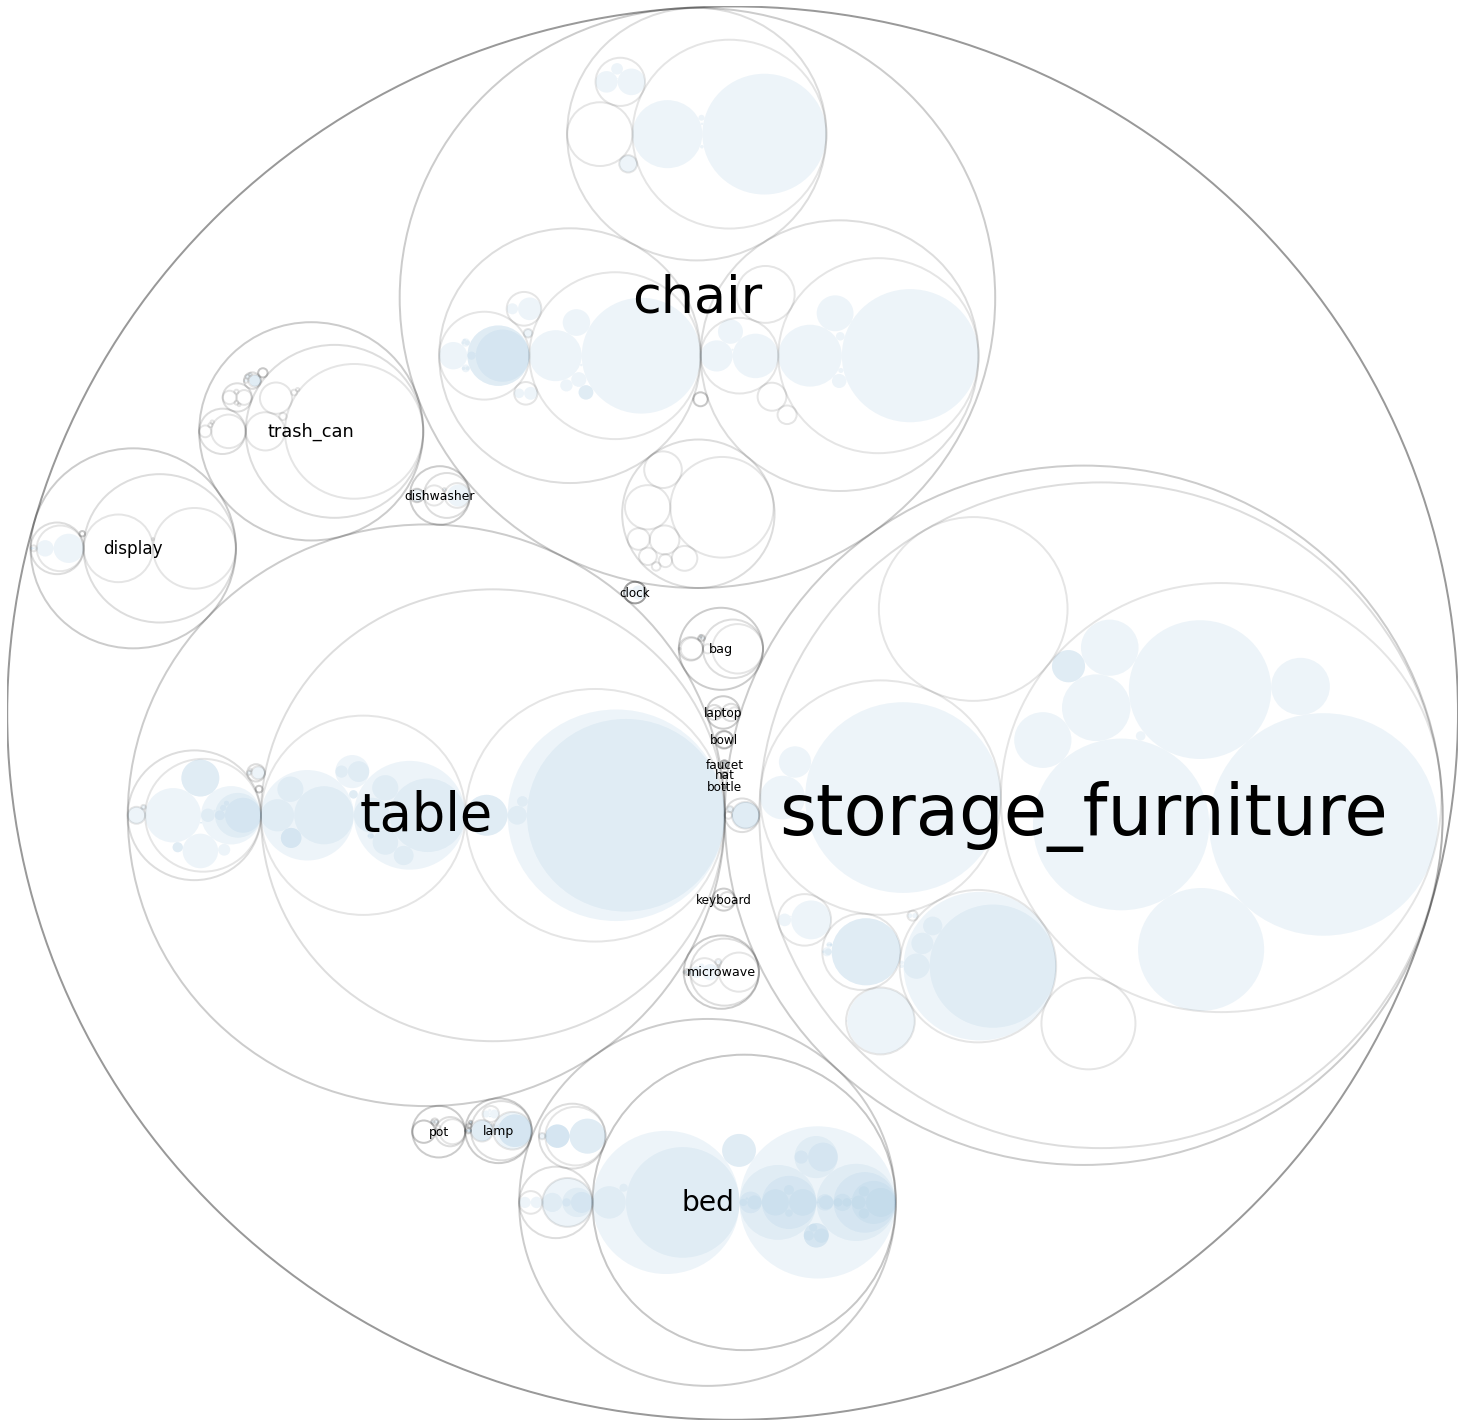
\includegraphics[trim=0 0 0 0, max width=\textwidth]{Figures/scan2part/treemap_v2.png}
% % trim=left bottom right top
% 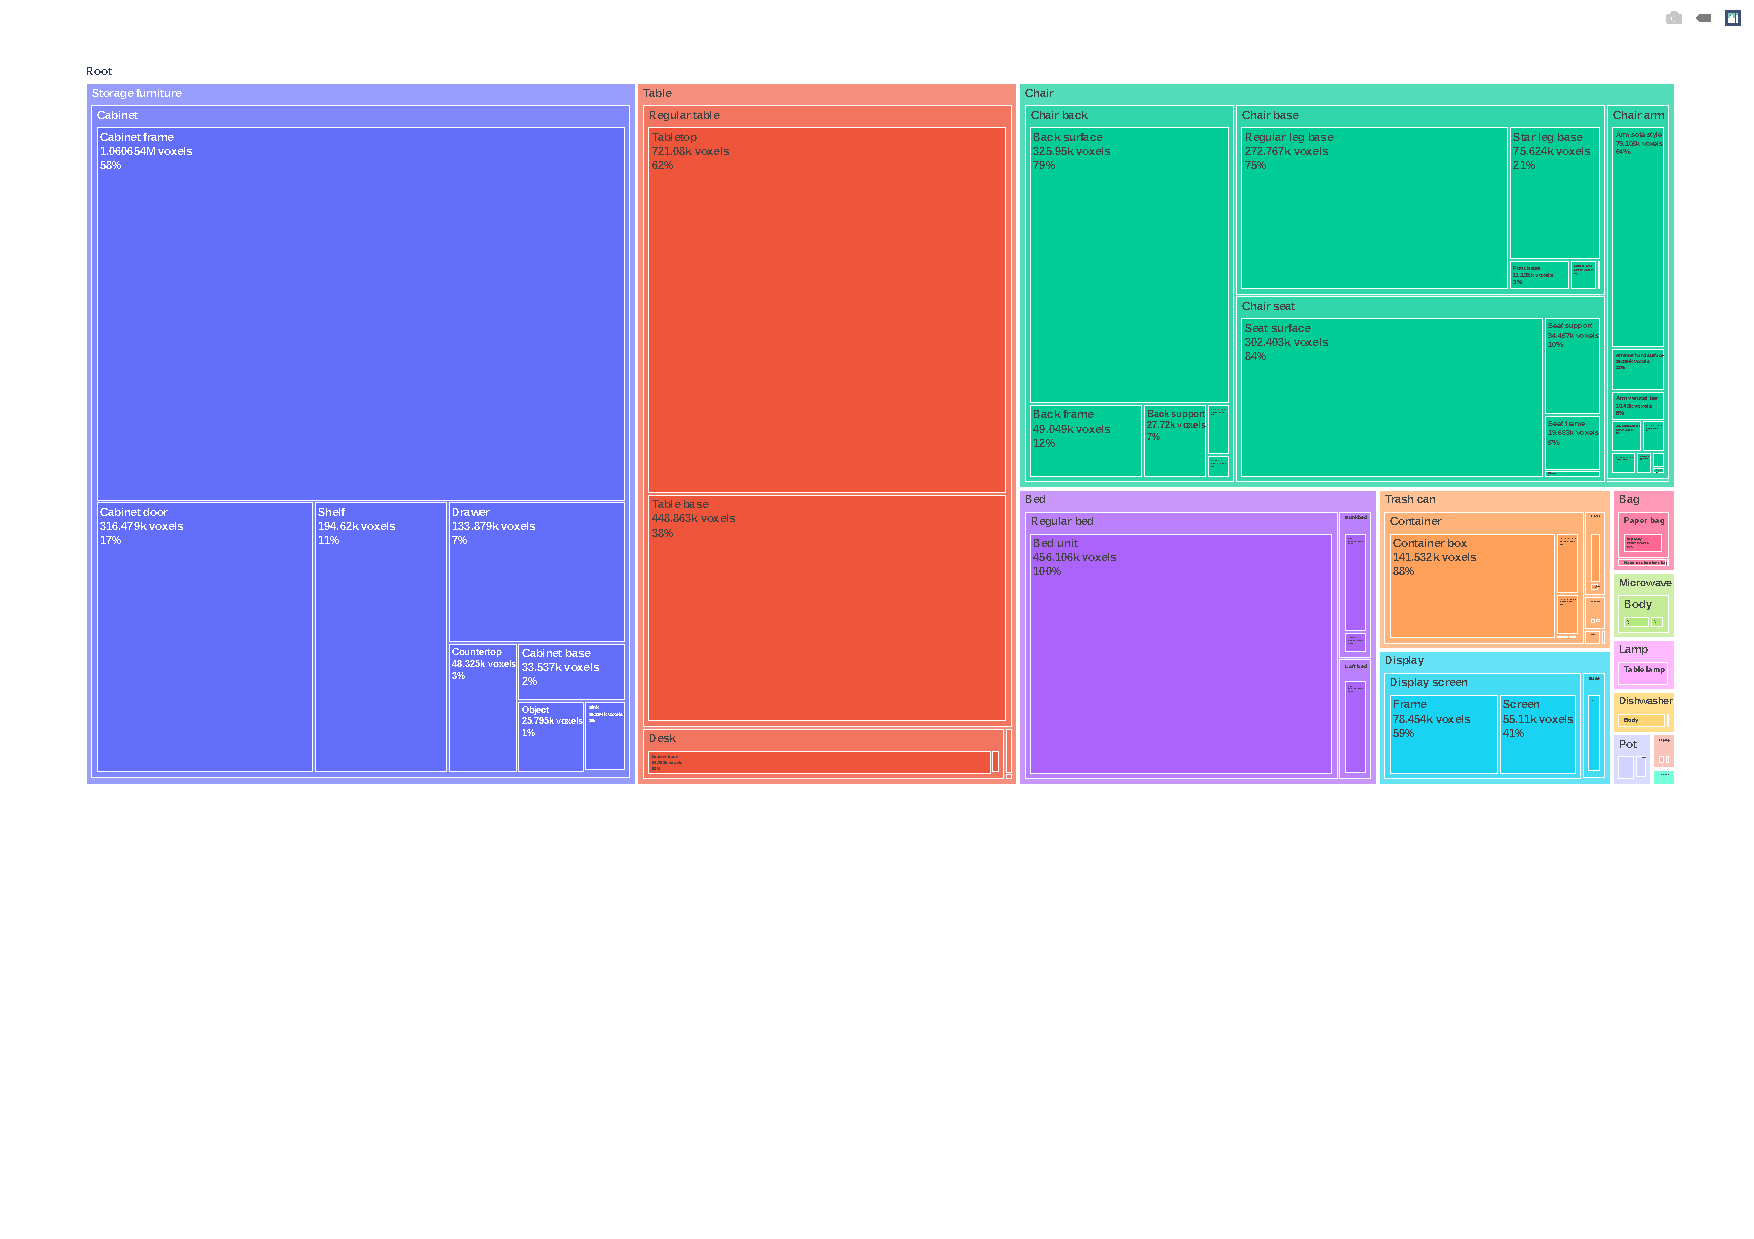
\includegraphics[trim=0 220 0 20, clip, max width=\textwidth]{Figures/scan2part/treemap_plot.pdf}
% \caption{Frequencies of classes in the part hierarchy. The areas of circles are proportional to the number of part voxels as a fraction of the number of voxels in the parent part.}
% \end{figure}


% \begin{figure}
% \label{fig:segmentation_architectures}
%   \centering
% 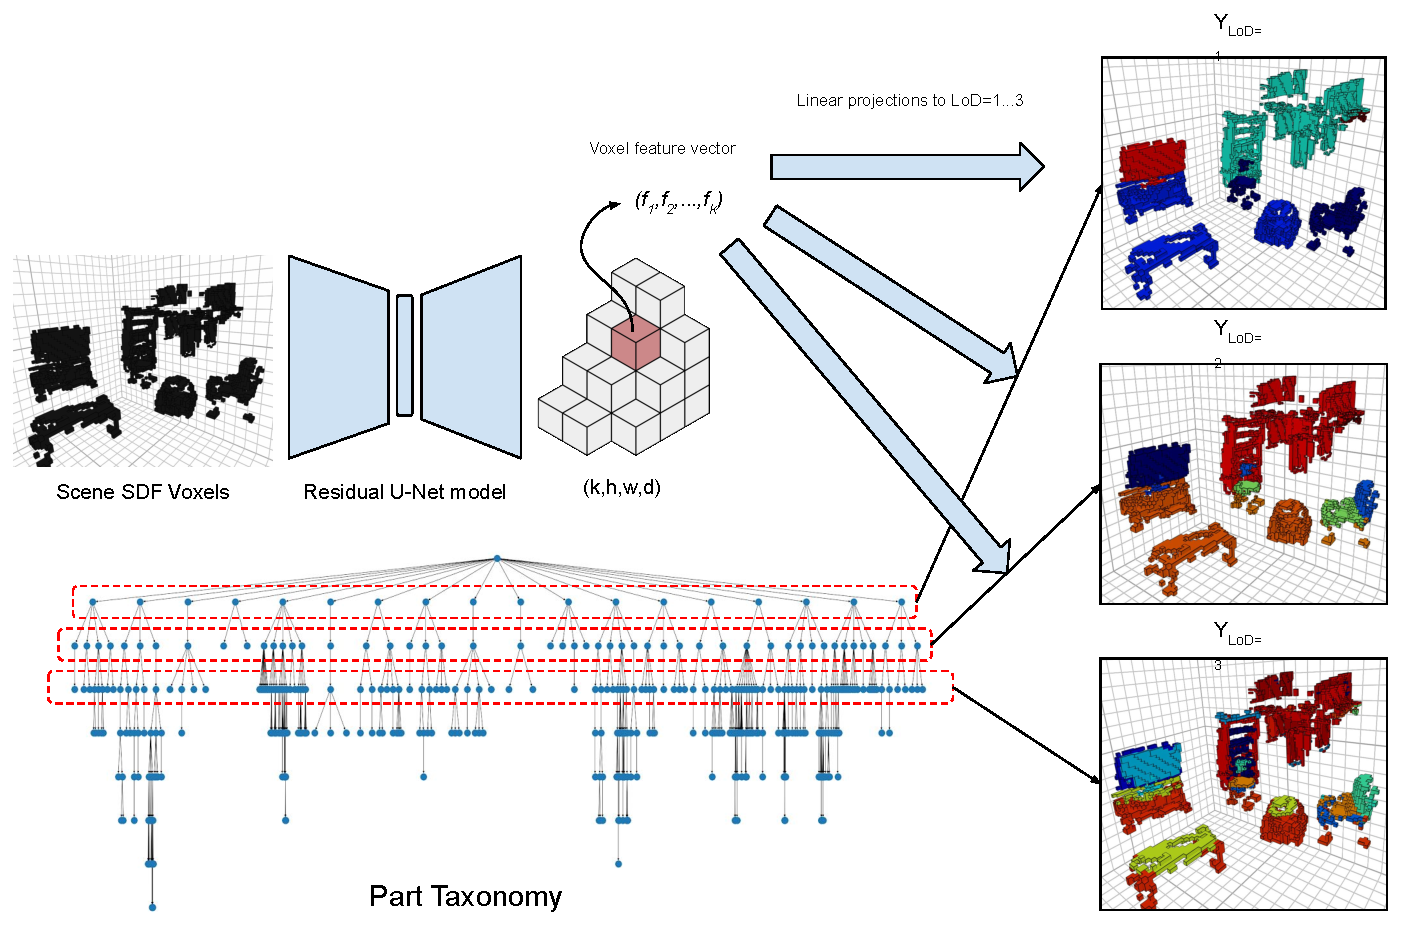
\includegraphics[trim=0 0 0 0, max width=\textwidth]{Figures/scan2part/architectures.pdf}
% \caption{Architectures of different segmentation models in different setups.}
% \end{figure}

% We compute a stratified train/test split, keeping split class ratios close to those in the whole dataset.
% Train and test sets were selected using combinatorial optimization routine that tries to split voxels of a class in ratios close to that of whole split.
We select 80\% of the scenes in ScanNet for training, keeping $1/16$ as a mini-validation to tune hyperparameters, and put aside 20\% scenes for testing.
During training, we extract 16~volumetric crops of size~$64^3$ from each voxelized scene and randomly shuffle them across all scenes in the training split.
% 16 crops were extracted from each scene, and shuffled with all other crops from other scenes.
The batch size we use ranges from 4 to 48 in different experiments, subject to fitting the network into the available GPU memory.
We optimize our models using Adam~\cite{kingma2014adam}, initalizing learning rate proportionally to the batch size, and decreasing it on pre-selected milestones by a factor $0.2$, with a weight decay of $10^{-4}$.
% for example for batch size = 32 base_lr=0.003, for bs=8 base_lr=0.001, for 48 base_lr=0.005 or 0.01 of it was too slow in training
We train until early stopping with patience parameter of 10, or until we reach a maximum epoch limit of 200.


% \DZ{unclear why different numbers where used}
% The encoder and the decoder consisted of 4 residual blocks each,  with output layers with  32 features for each voxel.
% Residual blocks included convolution, followed by ReLU non-linearity and group normalization with number of groups equal to 8.
% DZ already said this 
%Input tensors had only one channel the value of SDF function in that voxel.

\paragraph{Model configurations for different tasks}
\label{results:model_configs}
Table~\ref{table:configurations} summarizes our model specifications, differing by the choice of weights in~\eqref{eq:semseg_loss}.
To simplify the training process we assume all of the weights for loss functions to be normalized: $\sum_i \alpha_i = 1$.


\section{Experimental Results}
\label{sec:results}

\begin{wraptable}{r}{5.5cm}
\caption{Model configurations that we consider, with $\alpha_i$ in~\eqref{eq:semseg_loss}.}
\begin{tabular}{lrrr}\\\toprule  
Configuration   & $\alpha_1$ & $\alpha_2$ & $\alpha_3$ \\
\midrule
Base coarse     & 1 & 0 & 0 \\
Base middle     & 0 & 1 & 0 \\
Base fine       & 0 & 0 & 1 \\
MTT-12          & .5 & .5 &  0 \\
MTT-123-coarse  & .5 & .3 & .2 \\
MTT-123-fine    & .2 & .3 & .5 \\
\bottomrule
\end{tabular}
\label{table:configurations}
\end{wraptable} 

\paragraph{The choice of scene understanding levels. }
\label{results:levels}
We evaluate the algorithms at three granularity levels for each object category: coarse-, middle- and fine-grained, roughly corresponding to evaluation in~\cite{mo2019partnet}. 
Because of arbitrary nature of part labels in the PartNet dataset, metric scale doesn't always correspond to levels of object taxonomy. We choose to train on first 3 levels of object taxonomy to minimize discrepancy in geometry for levels >= 4.
Here are main guiding principles for levels of detail selection in a general case:
\begin{itemize}
    \item The higher the number of classes the lower segmentation performance of the model
    \item The higher the number of voxels for a given label class the higher prediction accuracy of that class
    \item The lower the level of detail the simpler geometry of parts on that level 
\end{itemize}

Trying to find the optimal trade-off between principle described above we concluded that all of the relevant information will be preserved if we work with hierarchy levels equal or lower than 3, and minimum number of voxels for a given class equal to 1800.

% TODO describe oracle and greedy mode, as equations, 


\paragraph{Quality measures. }
\label{results:metrics}
We evaluate semantic labeling and hierarchical segmentation models by inferring the semantic labels for entire input scenes and computing quality measures at each scene understanding level $d_k$ separately. 
More specifically, for each class $c$ present in the set of classes $\mathbb{C}_k$ at granularity $d_k$, we compute the standard Intersection over Union score $\text{IoU}_c$ and the balanced accuracy score $\text{Acc}_c$.
We report these per-class numbers along with mean IoU and mean balanced accuracy averaged over $\mathbb{C}_k$: $\text{mIoU}_k = \sfrac{1}{n_k}\sum_{c \in \mathbb{C}_k} \text{IoU}_c$, $\text{mAcc}_k = \sfrac{1}{n_k}\sum_{c \in \mathbb{C}_k} \text{Acc}_c$.

We additionally evaluate hierarchical semantic segmentation by averaging mIoU over all hierarchy levels $k \in \{1, \ldots, K\}$.

Instance segmentation is assessed as object detection and thus evaluate this task using average precision (AP) with IoU threshold at 0.5. To generate object hypotheses, each instance is checked against a threshold of confidence equal to 0.25, to filter out noisy voxels.

% Hierarchical models are evaluated somewhat differently. Specifically, we consider how categorical predictions of parts are combined to provide prediction of classes on some level of detail. 

% Ensemble models are evaluated by combining predictions either from different output "heads" of the model or from outputs of several separately trained models. 

% For Bottom-up approach - each "head" is evaluated separately, test set predictions are collected in a confusion matrix $C=(c_{ij}), i=1..N_C, j=1..N_C$, where $N_C$ is a number of classes of a certain "head". $TP_i = c_{ii}$ - is a number of true positives, $FP_i = \sum_{j=1..N_C} c_{ji} - TP_i$  is the number of false positives, and $FN_i = \sum_{j=1..N_C} c_{ij} - TP_i$ are false positive samples.
% We use the standard Intersection over Union (IoU) score defined as $\text{IoU}_c = \sfrac{TP_c}{(TP_c + FP_c + FN_c)}$ for class $c$ as well as a mean IoU.
% Balanced accuracy score~\cite{brodersen2010balanced} defined as average of per-class recall values $R_i$.
% \[
% R_i = \frac{TP_i}{TP_i + FN_i}
% \]
% is also computed. 

\paragraph{Part-level semantic labeling results. }
\label{results:semseg}
We first study part-level semantic labeling performance at different granularity levels $d_1, d_2, d_3$ in Table~\ref{tab:semseg}. 

We found that in some cases we can achieve a better performance than a baseline by evaluating model on lower level of details and projecting labels up through hierarchy. If $p_i^{d_j}$ - probability of a given voxel to have a class label $C_i^{d_j}$ where $i=1...n_j$ and $d_j, j=1, 2, 3$ - signifies the level of granularity, $Parent(i, d_j)$ - function that returns parent class index given child class index $i$ on the level $d_j$, because part hierarchy is a tree without isolated nodes, function always returns a single class index. Consequently the prediction labels projected up will be:
\begin{equation}
C_t^{d_{j-1}} = Parent\left(\argmax_{i=1...n_j}(p_i^{d_j}), d_j\right) .
\end{equation}

To improve prediction on a specific level of granularity we can train models in multitask setting which have shown their peak performance on multiple level of granularity. For example the MTT-12 and MTT-123-coarse have outperformed the base-coarse model on $d_1$, and the MTT-123-fine have outperformed base-fine model on $d_3$.
From that we can conclude that changing distribution of weights to different heads in multi-task setting trades performance across levels of details. Maximum value of weight in table~\ref{table:configurations} for the loss function term in~\eqref{eq:semseg_loss} roughly predicts level of detail with best performance.

\begin{figure}[!t]
\label{fig:experiments_visual}
\centering
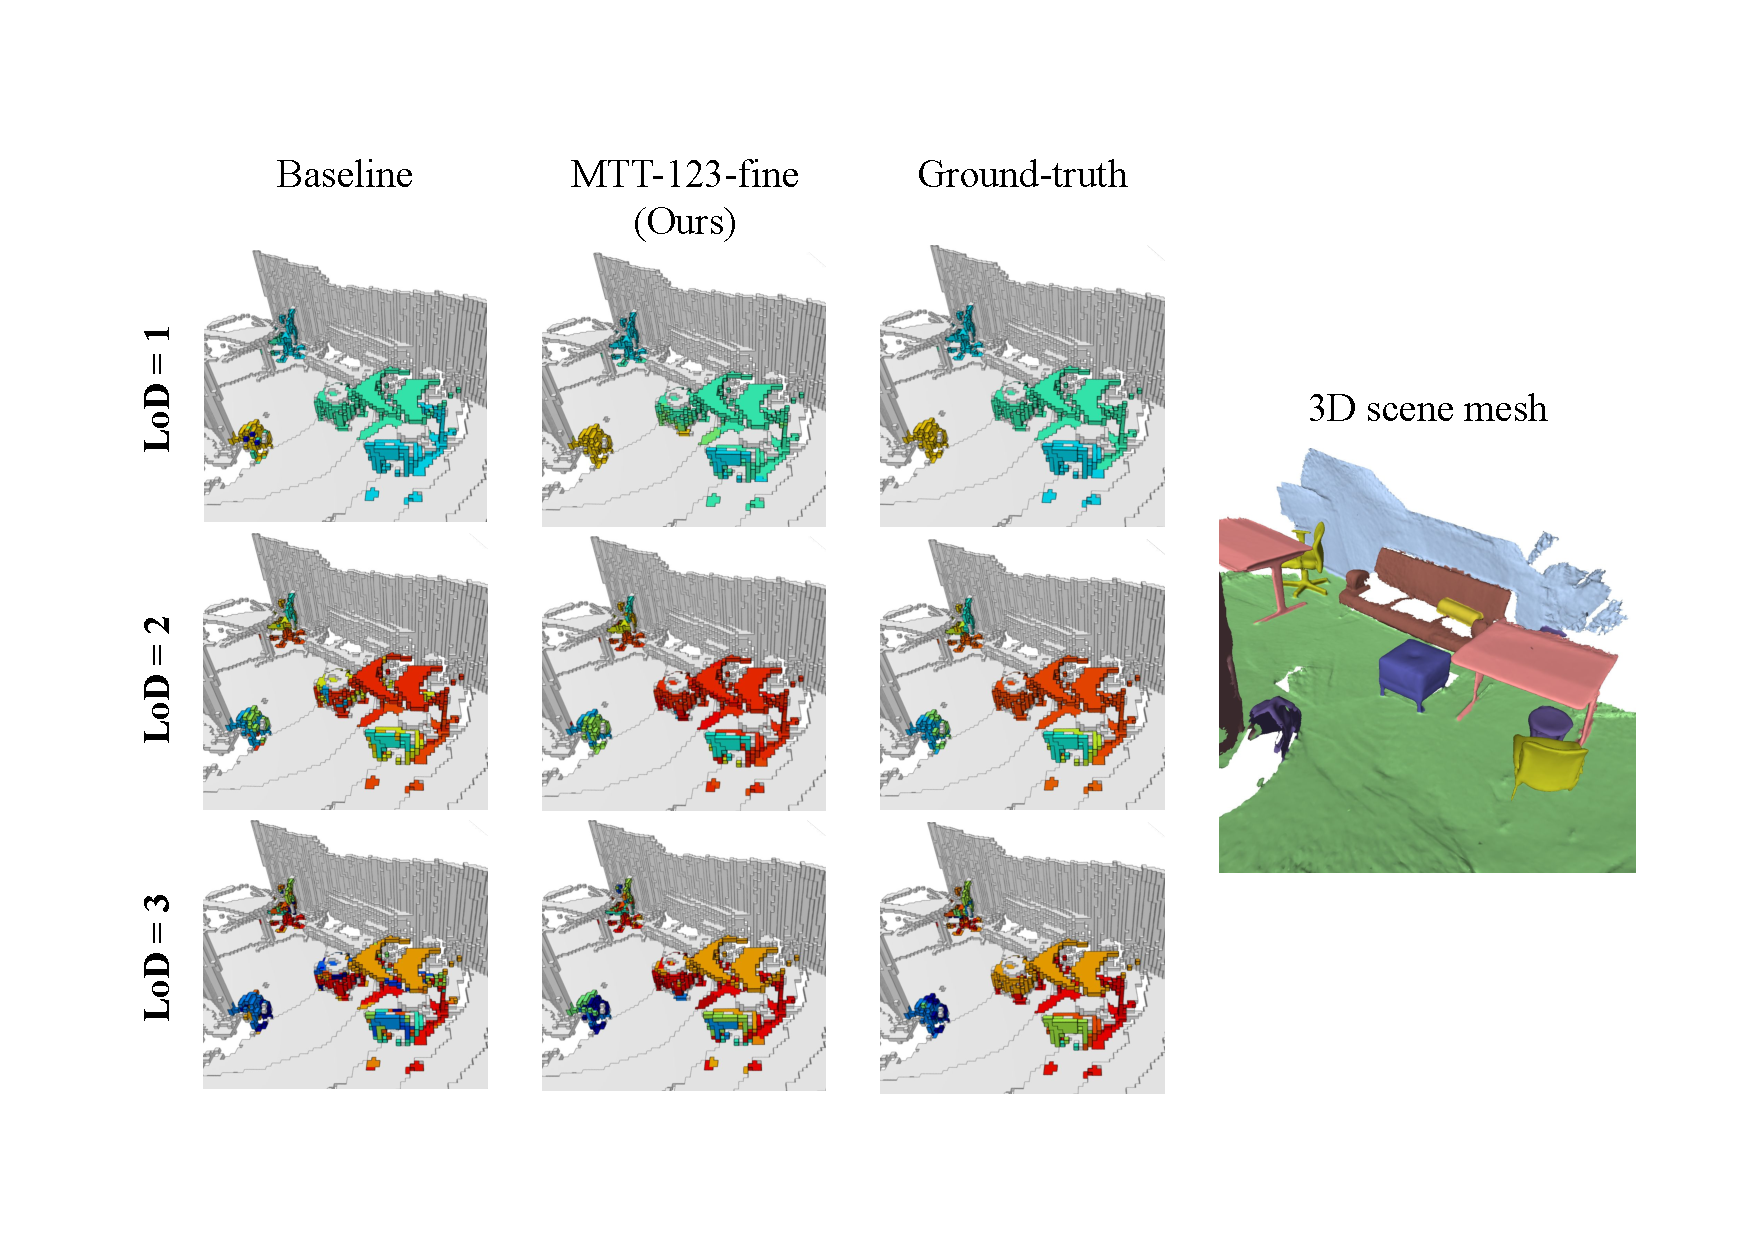
\includegraphics[width=0.99\textwidth]{Figures/scan2part/experiments_visual.pdf}
\caption{Qualitative hierarchical semantic segmentation results using the baseline models trained in each respective part-category level and our proposed method. Note the improved segmentation performance, particularly at finer levels in the parts taxonomy (lower row).}
\label{fig:hierarchical_seg_visual}
\end{figure}

\begin{table}[!h]

\caption{Part-level semantic segmentation performance in terms of mean IoU and mean balanced accuracy for different semantic granularities.}
\centering
\begin{tabular}{l rrr rrrr}
\toprule
 & \multicolumn{3}{c}{mAcc,\,\% $\uparrow$} && \multicolumn{3}{c}{mIoU,\,\% $\uparrow$} \\
\cmidrule{2-4}
\cmidrule{6-8}
Configuration   & $d_1$ & $d_2$ & $d_3$ && $d_1$ & $d_2$ & $d_3$ \\
\midrule
Base coarse     &  62.6 & ---   & ---   &&  22.5 & ---   & ---   \\
Base middle     &  \textbf{64.1} &  \textbf{57.9} & ---   &&  23.0 &  13.1 & ---   \\
Base fine       &  54.2 &  47.1 &  31.0 &&   9.5 &  \textbf{17.7} &   5.8 \\
% Base coarse (nw) & 71.74 & --- & --- & 27.15 & --- & --- \\
% Base coarse (bg) & 88.78 & --- & --- &  1.8  & --- & --- \\
\midrule
MTT-12          &  63.4 &  53.5 & ---   &&  \textbf{28.7} &  15.9 & ---   \\
MTT-123-coarse  &  63.5 &  56.2 &  32.5 &&  23.3 &  12.0 &   6.3 \\
MTT-123-fine    &  60.7 &  52.6 &  \textbf{34.7} &&  21.9 &  12.1 &   \textbf{6.7} \\
\midrule
Num. classes    &    13 &    36 &    79 &&    13 &    36 &    79 \\
\bottomrule
\end{tabular}
\label{tab:semseg}

\end{table}

\paragraph{Hierarchical semantic segmentation results. }
\label{results:hierarhical}
We present performance of hierarchical semantic segmentation in Table~\ref{tab:hierarchical_seg} and display these visually in Figure~\ref{fig:hierarchical_seg_visual}. Note that despite the baselines are focusing solely on their respective level of semantic detail, our methods is able to leverage a multi-task objective in~\eqref{eq:semseg_loss} to perform more efficient segmentation.

Hierarchical semantic segmentation is performed in a similar fashion to segmentation in MTT setting, but instead of classification of each voxel on each level of detail, heads in hierarchical model are more numerous (51 head) and perform classification of voxels to a specific sub-part class of parent class, e.g. classifying presumed chair shape to chair back, legs and seat. In this setting model is evaluated in two modes:
\begin{itemize}
    \item Oracle - in this mode mask of the parent class is taken from the ground truth data, thus each head is evaluated on it's ability to classify specific sub-parts of a certain object on specific level of detail. 
    \item Greedy - when parent object mask is predicted by heads higher in the hierarchy, predictions of the root node in hierarchy is performed first, masks for the objects are computed and heads lower on the tree evaluated only on respective mask. In this way model is evaluated as a whole top-down, which can lead to compounding of errors.
\end{itemize}
The results in Table~\ref{tab:hierarchical_seg} tell us that hierarchical model can segment specific sub-parts of many objects reasonably well. The problem arises when we try to integrate the predictions one after another in a sequential decision process, causing errors to compound and become incorrect the deeper in the tree they go.

\begin{table}[!h]

\caption{Hierarchical semantic segmentation results in terms of mean IoU and mean balanced accuracy for different semantic granularities. We include mIoU averaged over all hierarchy levels as an integral measure.}
\centering
\begin{tabular}{l rrrr r rrrr}
\toprule
  & \multicolumn{4}{c}{mAcc,\,\% $\uparrow$} 
 && \multicolumn{4}{c}{mIoU,\,\% $\uparrow$} \\
\cmidrule{2-5}
\cmidrule{7-10}
Configuration           & $d_1$ & $d_2$ & $d_3$ &  avg. && $d_1$ & $d_2$ & $d_3$ & avg. \\
\midrule
**Oracle (top-down)        &  58.5 &  82.0 &  70.9 &  70.5 &&   15.8 &  43.3 &  36.2& 31.8 \\
\midrule
Base fine (bottom-up)    &  54.2 &  47.1 &  31.0 &  44.1 &&   9.5 &  \textbf{17.7} &   5.8 & 11.0 \\
Greedy (top-down)        &  30.9 &  16.4 &   9.2 &  18.8 &&  19.0 &   9.2 &   4.8 & 11.0 \\
MTT-123-coarse           &  \textbf{63.5} &  56.2 &  32.5 &  50.7 &&  \textbf{23.3} &  12.0 &   6.3 & \textbf{13.9} \\
MTT-123-fine             &  60.7 &  52.6 &  34.7 &  49.4 &&  21.9 &  12.1 &  \textbf{6.7} & 13.6 \\
MTT-123-coarse (ensemble)&  \textbf{63.5} &	\textbf{56.8} &	33.8 & \textbf{51.4} &&   \textbf{23.3} &  11.6 &   6.1 & 13.7 \\
MTT-123-fine (ensemble)  & 60.7	 & 53.1 &	\textbf{35.6} & 49.8 &&   21.9 &  11.7 &   6.6 & 13.4 \\
\midrule
Num. classes            &    13 &    36 &    79 &       &&    13 &    36 &    79 &      \\
\bottomrule
\end{tabular}
\label{tab:hierarchical_seg}
\end{table}


\paragraph{Part instance segmentation results. }
\label{results:instance}
We present instance segmentation results in Table~\ref{table:instance}.

As expected performance of instance segmentation drops with reduction of level of detail, caused mainly by the loss of the unique properties of the instance masks, and lowering of the mean number of the voxels per instance mask.

Because we have $d_1$ level object instance mask and semantic part masks, to create $d_2, d_3$ instance masks we have a pre-processing step that selects unique semantic masks for each object instance mask separately.

\begin{table}[!h]

\caption{Instance segmentation performance in terms of mean IoU for varying levels of detail (LoD).}
\centering
\begin{tabular}{lrrr}
\toprule
Configuration       & mIoU,\,\% & AP@50,\,\%    & AR@50,\,\% \\ 
\midrule
Base coarse         & \textbf{78.6}     & \textbf{83.9} & \textbf{35.9} \\
% LoD=1, bg-push & \textbf{80.56\%} & 74.50\% & \textbf{37.11\%} \\
Base middle         & 70.5     & 54.2         & 16.6 \\
Base fine           & 64.7     & 41.4         & 15.4 \\
\bottomrule
\end{tabular}%
\label{table:instance}

\end{table}



\section{Conclusion}
We introduced a challenging benchmark for individual parts segmentation of objects in real-world, noisy indoor environments and a novel dataset Scan2Part to evaluate on. 
The core of our method is to leverage structural knowledge of objects composition to perform a variety of segmentation tasks in setting with complex geometry, high levels of uncertainty due to noise. To achieve that, we explore the part taxonomies of common objects in indoor scenes, on multiple scales and methods of compressing them for more effective use in machine learning applications. We demonstrated that specific ways of training deep segmentation models like ours Residual-U-Net style architecture are better at capturing inductive biases in structured labels on some parts of a taxonomy but not the others. Further research on relationships between structure of real-world scenes and perception models is required and we hope our benchmark and dataset will accelerate it.  


\section*{Broader Impact}
% Highlight both benefits and risks from your research. 
An obvious benefit of our research is the improved ability of automated systems to interact with complex environments which require perception on different spatial scales. It is also makes possible to extract more value from data gathered using commodity hardware like RGB-D sensors and modern smartphones. Possible risk that arises from application of technology based on our research is people relying on systems with assumption that algorithms have the same affordances as people.
% Highlight uncertainties
Composition properties of objects, parts and materials are diverse and depend on the culture, but less so with emergence of globalised manufacturing.  

\todo{add main.supp.tex}
% \subsubsection*{Acknowledgments}
% Use unnumbered third level headings for the acknowledgments. All
% acknowledgments, including those to funding agencies, go at the end of the paper.

% \clearpage


% \bibliographystyle{nips}
% \bibliography{references}


% \clearpage


% \appendix
% \section{Full results of Segmentation models}

\begin{table}[!htb]
\caption{Full dataset and testset statistics. As you can see it's highly unbalanced.}
\resizebox{\textwidth}{!}{%
\begin{tabular}{l|lllll}
classes & \% in testset & \# voxel & \% voxels & \# scenes & \# inst. in testset\\ \hline
Microwave & 18.75\% & 20141 & 0.38\% & 90 & 21\\
Display & 19.36\% & 149988 & 2.84\% & 350 & 142\\
Lamp & 20.14\% & 15736 & 0.30\% & 95 & 26\\
Laptop & 19.95\% & 3950 & 0.07\% & 46 & 11\\
Bag & 19.75\% & 25225 & 0.48\% & 136 & 33\\
Storage & 19.41\% & 1833826 & 34.68\% & 866 & 496\\
Bed & 20.94\% & 504774 & 9.55\% & 271 & 69\\
Table & 20.82\% & 1268401 & 23.99\% & 1104 & 539\\
Chair & 16.95\% & 1261928 & 23.87\% & 960 & 754\\
Dishwasher & 20.99\% & 12846 & 0.24\% & 24 & 6\\
TrashCan & 18.96\% & 178648 & 3.38\% & 634 & 199\\
Vase & 20.48\% & 9989 & 0.19\% & 30 & 9\\
Keyboard & 19.63\% & 1819 & 0.03\% & 24 & 9\\
% Bowl & 28.86\% & 1178 & 0.02\% & 12 \\
% Faucet & 2.44\% & 246 & 0.00\% & 4 \\
% Clock & 12.28\% & 1742 & 0.03\% & 15 \\
% Hat & 100.00\% & 101 & 0.00\% & 1 \\
% Bottle & 0.00\% & 23 & 0.00\% & 1
\end{tabular}%
\label{tab:datasetstats}
}
\end{table}

% Please add the following required packages to your document preamble:
% \usepackage{graphicx}
{\lat
\begin{table}[!htb]
\caption{mIoU of different models for each class}
\resizebox{\textwidth}{!}{%
\begin{tabular}{l|llllll}
Classes & Original & bg & no-w & LoD=1-2 & LoD=1-3, Dec & LoD=1-3, Inc \\
\hline
Microwave & 2.05\% & 0.52\% & 3.41\% & \textbf{15.86\%} & 4.74\% & 7.99\% \\
Display & 42.28\% & 1.69\% & 41.44\% & \textbf{44.10\%} & 39.94\% & 39.01\% \\
Lamp & 17.10\% & 0.64\% & \textbf{21.85\%} & 17.81\% & 16.47\% & 9.62\% \\
Laptop & 9.80\% & 1.07\% & 5.60\% & 11.64\% & \textbf{11.91\%} & 6.91\% \\
Bag & 9.97\% & 0.78\% & 4.23\% & \textbf{11.42\%} & 7.39\% & 5.98\% \\
Storage & 47.18\% & 2.91\% & \textbf{63.40\%} & 47.10\% & 55.97\% & 44.29\% \\
Bed & 31.98\% & 5.60\% & \textbf{53.70\%} & 46.27\% & 32.73\% & 32.78\% \\
Table & 49.21\% & 3.96\% & \textbf{53.52\%} & 50.73\% & 46.14\% & 47.74\% \\
Chair & 55.13\% & 3.73\% & 65.86\% & \textbf{69.67\%} & 54.07\% & 62.05\% \\
Dishwasher & 0.00\% & 0.00\% & \textbf{8.68\%} & 0.10\% & 0.28\% & 0.00\% \\
TrashCan & 21.35\% & 1.94\% & 28.98\% & \textbf{40.64\%} & 18.46\% & 25.80\% \\
Vase & 1.83\% & 0.03\% & 2.00\% & \textbf{9.84\%} & 2.72\% & 1.00\% \\
Keyboard & 4.06\% & 0.53\% & 0.26\% & 8.15\% & \textbf{11.74\%} & 1.27\% \\
\hline
mIoU & 22.46\% & 1.80\% & 27.15\% & \textbf{28.72\%} & 23.27\% & 21.88\%
\end{tabular}%
\label{tab:lodmiou1table}
}
\end{table}}

{\lat
\begin{table}[!htb]
\caption{results of the models on Instance Segmentation task, original model and with background push}
\resizebox{\textwidth}{!} & \textbf{87.50\%} & \textbf{33.33\%} & 80.59\% & 75.00\% & 28.57\% \\
Display & \textbf{76.15\%} & \textbf{64.62\%} & 29.58\% & 73.59\% & 64.00\% & \textbf{33.80\%} \\
Lamp & 65.29\% & 75.00\% & \textbf{34.62\%} & \textbf{70.64\%} & \textbf{77.78\%} & 26.92\% \\
Laptop & \textbf{50.44\%} & \textbf{100.00\%} & \textbf{9.09\%} & NaN & 0.00\% & 0.00\% \\
Bag & 89.19\% & \textbf{100.00\%} & \textbf{33.33\%} & \textbf{91.70\%} & 75.00\% & 27.27\% \\
Storage & \textbf{82.01\%} & 71.71\% & 37.30\% & 81.44\% & \textbf{74.70\%} & \textbf{38.10\%} \\
Bed & \textbf{79.55\%} & 62.86\% & 63.77\% & 78.38\% & \textbf{74.29\%} & \textbf{75.36\%} \\
Table & 77.34\% & 77.10\% & 42.49\% & \textbf{80.35\%} & \textbf{81.37\%} & \textbf{46.20\%} \\
Chair & 82.88\% & 82.14\% & 30.50\% & \textbf{86.01\%} & \textbf{86.79\%} & \textbf{32.23\%} \\
Dishwasher & 71.32\% & 100.00\% & 66.67\% & \textbf{72.66\%} & \textbf{100.00\%} & \textbf{66.67\%} \\
TrashCan & 87.22\% & \textbf{86.18\%} & \textbf{53.27\%} & \textbf{89.88\%} & 85.12\% & 51.76\% \\
Vase & \textbf{90.83\%} & 100.00\% & 33.33\% & 80.89\% & \textbf{100.00\%} & \textbf{55.56\%} \\
\hline
mIoU / mAP & 78.60\% & \textbf{83.93\%} & 35.94\% & \textbf{80.56\%} & 74.50\% & \textbf{37.11\%}
\end{tabular}%
\label{tab:lod1instsegresults}
}
\end{table}}


\begin{figure}[!htb]
\centering
\label{fig:partnet_to_scannet_labeling}
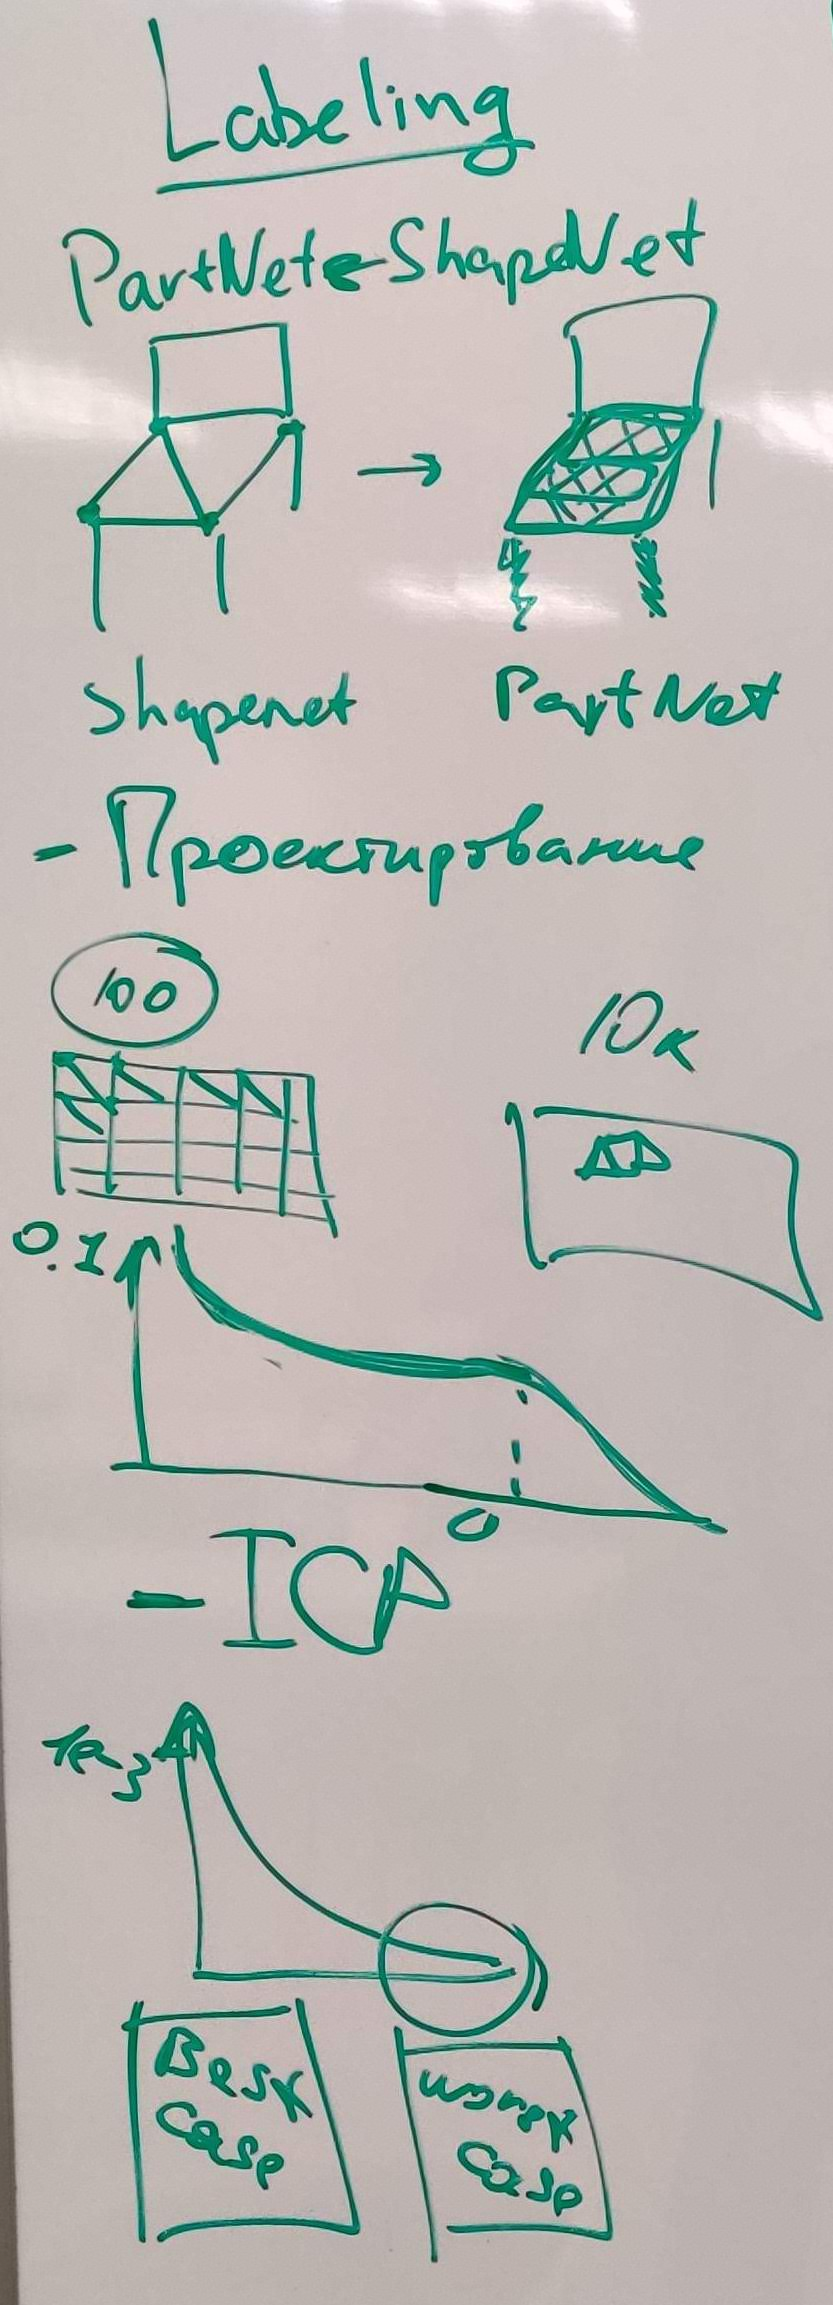
\includegraphics[trim=0 0 0 0, max width=0.25\textwidth]{images/partnet_to_scannet_labeling.jpg}
\caption{partnet to scannet labeling (a,b,c)}
% \end{wrapfigure}
\end{figure}

\begin{figure}[!htb]
\label{fig:scannet_overview}
  \centering
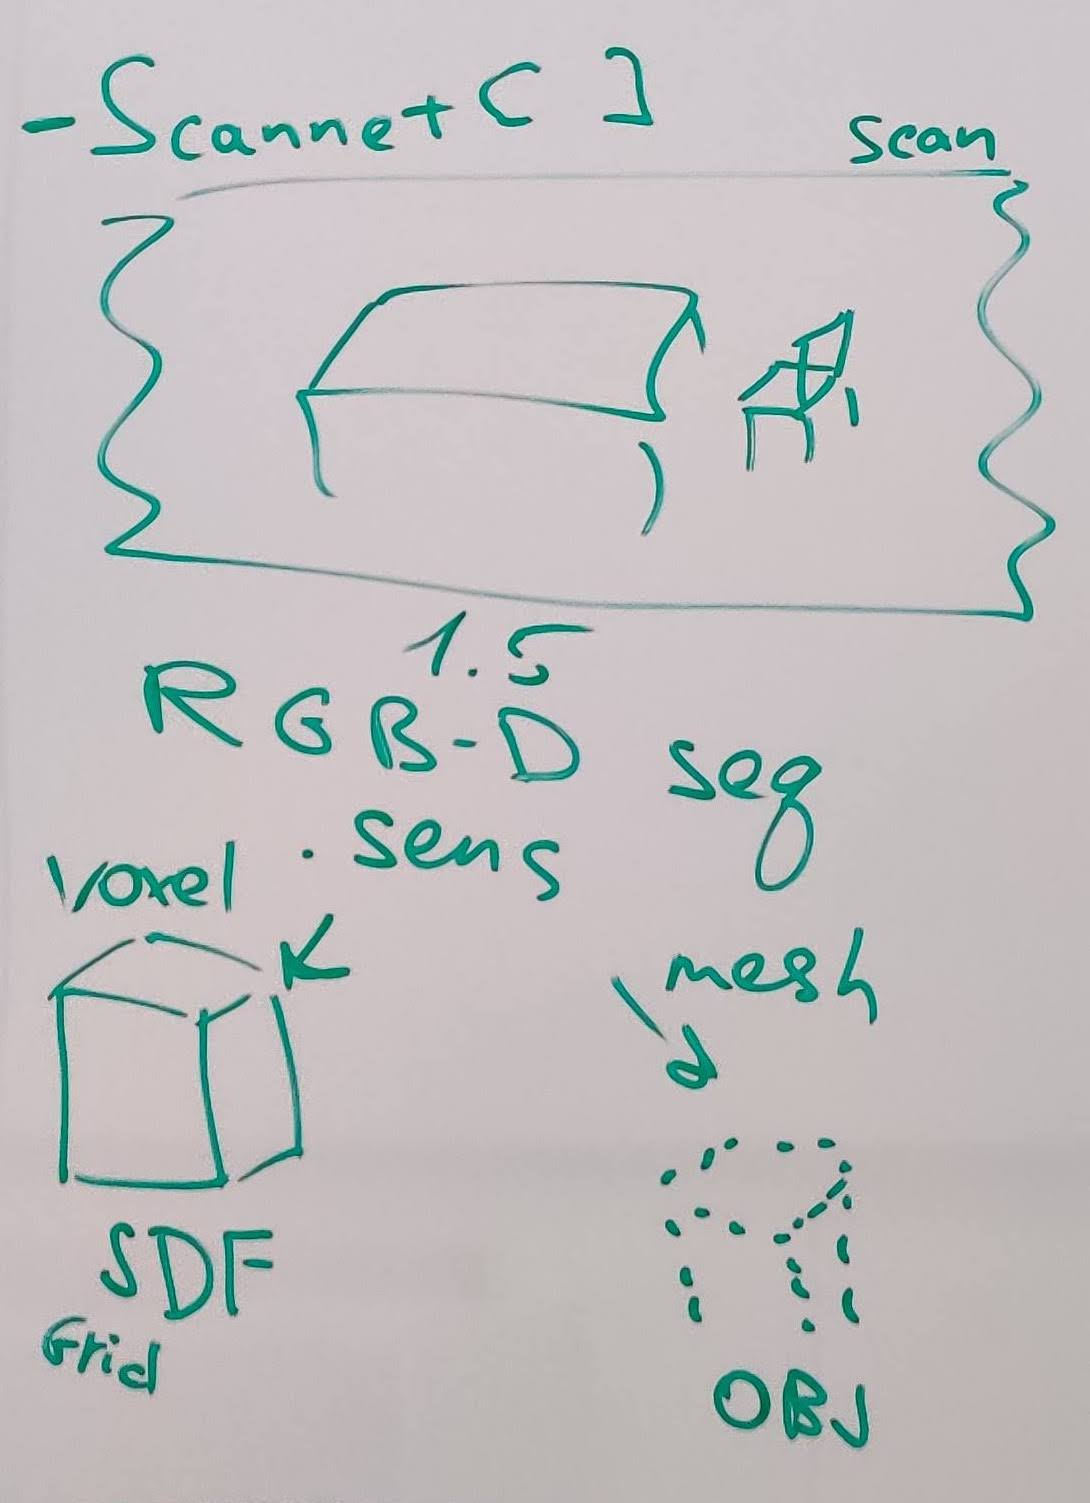
\includegraphics[trim=0 0 0 0, max width=0.5\textwidth]{images/scannet_overview.jpg}
\caption{scannet overview}
\end{figure}

\begin{figure}[!htb]
\label{fig:Scan2Cad_overview}
\centering
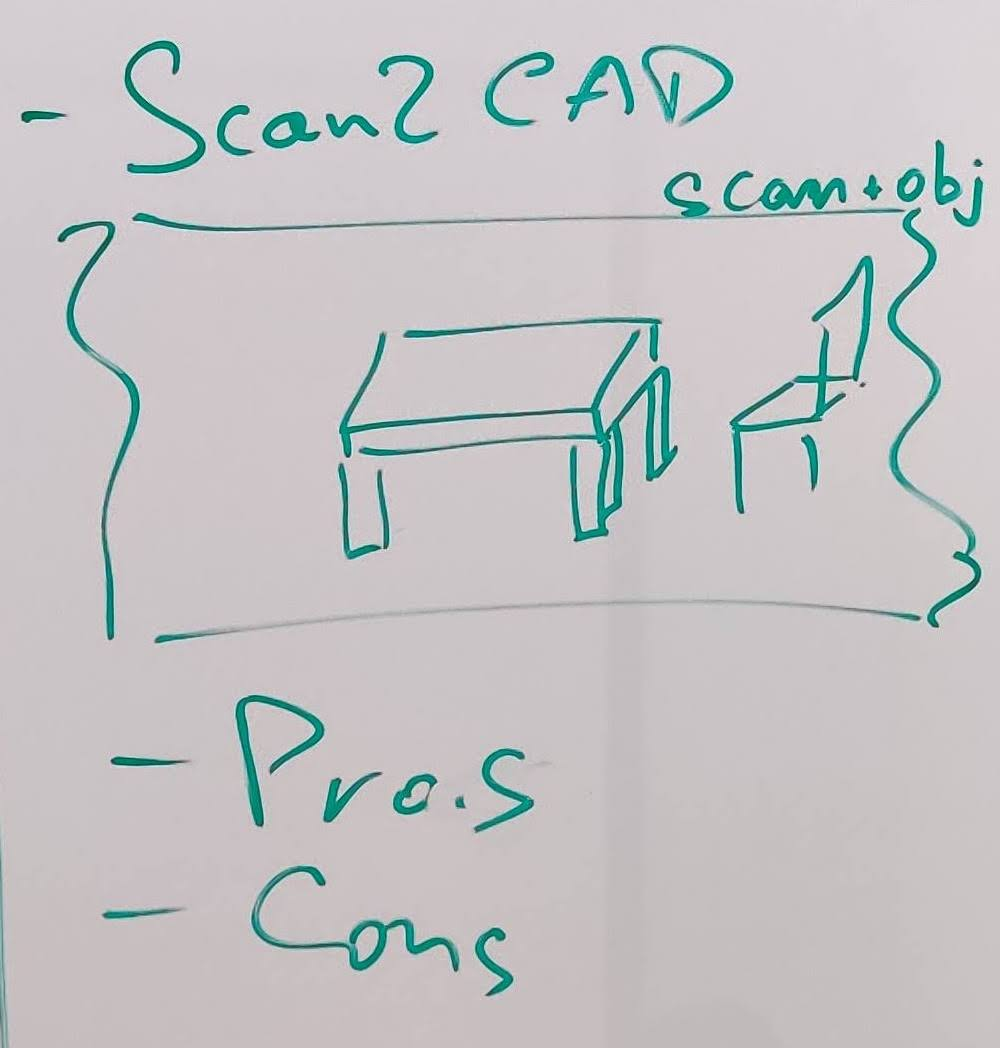
\includegraphics[trim=0 0 0 0, max width=0.5\textwidth]{images/Scan2Cad_overview.jpg}
\caption{Scan2Cad overview}
\end{figure}



\begin{table}[]
\caption{Proportions of ShapeNet semantic classes present in Scan2Cad dataset}
\label{table:scan2part_proportions}
\begin{tabular}{l|l|l}
Class ID & overlap? & class name \\
\hline
04379243 & 99.0\% (822/830) & table \\ \hline
02747177 & 98.9\% (88/89) & ashcan,trash can,garbage can,wastebin,ash bin,ash-bin \\ \hline
03211117 & 97.6\% (161/165) & display,video display \\ \hline
03761084 & 97.3\% (36/37) & microwave,microwave oven \\ \hline
03337140 & 97.1\% (68/70) & file,file cabinet,filing cabinet \\ \hline
03001627 & 96.9\% (632/652) & chair \\ \hline
02871439 & 96.7\% (145/150) & bookshelf \\ \hline
02933112 & 94.8\% (294/310) & cabinet \\ \hline
02818832 & 94.0\% (47/50) & bed \\ \hline
03991062 & 91.7\% (11/12) & pot,flowerpot \\ \hline
03207941 & 85.7\% (12/14) & dishwasher,dish washer,dishwashing machine \\ \hline
03085013 & 81.8\% (9/11) & computer keyboard,keypad \\ \hline
03325088 & 57.1\% (4/7) & faucet,spigot \\ \hline
02876657 & 50.0\% (1/2) & bottle \\ \hline
02808440 & 26.0\% (25/96) & bathtub,bathing tub,bath,tub \\ \hline
02801938 & 9.4\% (3/32) & basket,handbasket \\ \hline
04256520 & 8.1\% (20/247) & sofa,couch,lounge \\ \hline
02946921 & 0.0\% (0/1) & can,tin,tin can \\ \hline
03938244 & 0.0\% (0/5) & pillow \\ \hline
02828884 & 0.0\% (0/28) & bench \\ \hline
04554684 & 0.0\% (0/37) & washer,automatic washer,washing machine \\ \hline
03928116 & 0.0\% (0/25) & piano,pianoforte,forte-piano \\ \hline
03790512 & 0.0\% (0/4) & motorcycle,bike \\ \hline
03691459 & 0.0\% (0/2) & loudspeaker,speaker,speaker unit,loudspeaker system \\ \hline
03467517 & 0.0\% (0/6) & guitar \\ \hline
04330267 & 0.0\% (0/36) & stove \\ \hline
04401088 & 0.0\% (0/1) & telephone,phone,telephone set \\ \hline
04004475 & 0.0\% (0/31) & printer,printing machine \\ \hline
Total:    & 81.2\% (2477/3049) &         \\
\end{tabular}
\end{table}




\subsection{Scene labeling}

\textbf{PartNet -> Shapenet.} The PartNet \cite{mo2019partnet} is a hierarchical instance-level parts dataset of labels for the subset of the ShapeNet database. The PartNet dataset is the only dataset that has a deep hierarchical structure compared to other part annotation datasets, e.g.,  \cite{Yi16}. However, the PartNet dataset does not preserve the original ShapeNet coordinate system in the sense that each object is rotated in an unspecified order. For mapping labels to Scannet scenes, we need to restore the original coordinate system. To find the rotation matrix between coordinate systems, we use the following alignment process for each object: \begin{enumerate}
    \item we sample 20 different rotation angles corresponding to the vertices of the convex regular dodecahedron;
    \item each rotation angle is represented as the initial alignment matrix of the object for alignment;
    \item we perform Point-to-point ICP alignment separately for each initial alignment matrix;
    \item we select the best one out of 20 alignment results where the distance between the original ShapeNet shape and the rotated PartNet shape is minimal.
\end{enumerate}

\textbf{Shapenet -> Scannet (Scan2CAD).} The Scan2CAD \cite{avetisyan2019scan2cad} is a dataset that aligns CAD objects from ShapeNet \cite{chang2015shapenet} database to scenes from Scannet. Using the marching cubes algorithm, we obtained  voxelized versions of scenes from ScanNet dataset with object type labels and mapping of coordinate systems from ScanNet to ShapeNet.  Finally, we  calculate the position of CAD object parts in the scene coordinate system and calculate relative volume in specific voxels thus projecting part labels on the scene. \DZ{unclear what relative volume is needed for here}

Under closer examination, we discovered that most of the parts do not have a unique shape making the task of instance segmentation for parts very hard to solve and not necessary for practical scene segmentation task. \DZ{unclear}



% \end{document}